%-----------------------------------------------------------------------------
%
%               Template for LaTeX Class/Style File
%
% Name:         sigplanconf-template.tex
% Purpose:      A template for sigplanconf.cls, which is a LaTeX 2e class
%               file for SIGPLAN conference proceedings.
%
% Author:       Paul C. Anagnostopoulos
%               Windfall Software
%               978 371-2316
%               paul@windfall.com
%
% Created:      15 February 2005
%
%-----------------------------------------------------------------------------


\documentclass[preprint]{sigplanconf}

\usepackage{amsmath}
\usepackage{url}
\usepackage{xspace}
\usepackage{alltt}
\usepackage{verbatim}
%\usepackage{color}
%\usepackage[dvips]{epsfig}
\usepackage[pdftex]{graphicx}

\newcommand{\ocamlgraph}{\textsc{Ocamlgraph}\xspace}
\newcommand{\ocaml}{\textsc{Ocaml}\xspace}
\newcommand{\fl}{\ensuremath{\rightarrow}}

\begin{document}

\conferenceinfo{GPCE '06}{October 22--26 2006, Portland, Oregon.} 
\copyrightyear{2006} 
\copyrightdata{[to be supplied]} 

\titlebanner{}        % These are ignored unless
\preprintfooter{}   % 'preprint' option specified.

\title{Designing a Generic Graph Library using ML Functors}
\subtitle{}

\authorinfo{Submitted for blind review}{}{}
%\authorinfo{S. Conchon\and J.-C. Filli\^atre\and J. Signoles}
%           {LRI Universit\'e Paris Sud 91405 Orsay France}
%           {\{conchon,filliatr,signoles\}@lri.fr}

\maketitle

\begin{abstract}
  This article details the design and implementation of \ocamlgraph, a
  generic graph library for the programming language \ocaml. This
  library features a large set of graph data structures---directed or
  undirected, with or without labels on vertices and edges, as persistent
  or mutable data structures, etc.---and a large set of graph
  algorithms written independently of the graph data structure. Such a
  genericity is obtained through a massive use of \ocaml module system
  and of its functions, the so-called \emph{functors}.
\end{abstract}

\category{D.2}{Software Engineering}{Software Architectures; Design;
  Reusable Software}

%\terms
%term1, term2

\keywords
Graph library, Generic programming, Functors

\section{Introduction}

Finding a graph library for one's favorite programming language is
usually easy. But using the provided algorithms on one's
own graph data structure or building undirected persistent graphs with
vertices and edges labeled with something else than integers is
likely to be more difficult.

This article introduces
\ocamlgraph\footnote{\url{http://www.lri.fr/~filliatr/ocamlgraph/}}, a
generic graph library for the programming language
\ocaml~\cite{ObjectiveCaml}. Beside the mere presentation of this
library, this article demonstrates how \ocaml has been used to
introduce genericity at two levels in this library. First, \ocamlgraph
does not provide a single data structure for graphs but many of them,
enumerating all possible variations---directed or undirected graphs,
persistent or mutable data structures, user-defined labels on vertices
or edges, etc.---under a common interface.
Second, \ocamlgraph provides a large set of graph algorithms that are
written independently of the underlying graph data structure. Then
they can be applied on the data structures provided by \ocamlgraph
itself but also on user-defined data structures as soon as they
implement a minimal set of functionalities.

The genericity of \ocamlgraph, on both levels of data structures and
algorithms, is realized through a massive use of \ocaml module
system~\cite{leroy00}. In the first case, it is used to avoid code
duplication between the many variations of graph data structures,
which is mandatory here seen the high number (19) of similar but all
different implementations. In the second case, it is used to write
the graph algorithms independently of the underlying graph data
structure, with as much genericity as possible but also with an
efficiency concern in mind. In both cases, the technical solution
comes from the functions of \ocaml module system, the so-called
\emph{functors} in the functional programming jargon (that should not
be confused with C++ functors). This article aims at explaining these
two different uses of functors and thus is more a software engineering
article than a graph library description.

This article is organized as follows. Section~\ref{systememodules}
briefly introduces the \ocaml module system. Then
Section~\ref{structuresdedonnees} exposes the design of the common
interface for all graph data structures and explains how the code is
shared among the various implementations. Section~\ref{algos}
describes the algorithms provided in \ocamlgraph and how the
genericity with respect to the graph data structure is obtained.
Section~\ref{exemples} illustrates the use of \ocamlgraph\ on two
typical situations.  Finally Section~\ref{bench} presents some
benchmarks and Section~\ref{comparaison} compares \ocamlgraph with
several existing graph libraries.

\section{\ocaml Module System}\label{systememodules}

This section quickly describes the \ocaml module system. Any reader
familiar with \ocaml can safely skip this section.

The module system of \ocaml is a language by itself, on top of the
core \ocaml language, which only fulfills software engineering
purposes: separate compilation, names space structuring, encapsulation
and genericity. This language appears to be independent of the core
language~\cite{leroy00} and may be unfolded statically.  It is a
strongly typed higher-order functional language. Its terms are called
\emph{modules} or \emph{structures}.  They are the basic blocks in
\ocaml programs, that package together types, values, exceptions
and sub-modules. 

\subsection{Structures}

Modules are introduced using the \texttt{struct...end} construct and
the (optional) \texttt{module} binding is used to give them a name.
Outside a module, its components can be referred to using the
\emph{dot notation}: \texttt{M.c} denotes the component
\texttt{c} defined in the module \texttt{M}.

For instance, a module packaging together a type for a graph data
structure and some basic operations can be implemented in the
following way:
\begin{alltt}
module Graph = struct
  type label = int 
  type t = (int * label) list array
  let create n = Array.create n []
  let add_edge g v1 v2 l = g.(v1) <- (v2,l)::g.(v1)
  let iter_succ g f v = List.iter f g.(v)
end
\end{alltt}
The type \texttt{Graph.t} defines a naive graph data structure using
adjacency lists with edges labeled with integers: a graph is an array
(indexed by integers representing vertices) whose elements are lists of
pairs of integers and labels (declared as an alias for the type
\texttt{int}). 

\subsection{Signatures}

The type of a module is called a \emph{signature} or an
\emph{interface}\footnote{with the same meaning as in \textsc{Modula}
  but not as in \textsc{Java}} and can be used to hide some components
or the definition of a type (then called an \emph{abstract data
  type}). Signatures are defined using the \texttt{sig...end}
construct and the (optional) \texttt{module type} binding is used to
give them a name. Constants and functions are declared 
via the keyword \texttt{val} and types via the keyword \texttt{type}.

For instance, a possible signature for the \texttt{Graph} module
above, that hides the graph representation and the type of labels,
could be the following:
\begin{alltt}
module type GRAPH = sig
  type label
  type t
  val create : int -> t
  val add_edge : t -> int -> int -> label -> unit 
  val iter_succ : 
    t -> (int * label -> unit) -> int -> unit
end
\end{alltt}
Restricting a structure by a signature results in another view of the
structure. This is done as follows:
\begin{alltt}
module G' = (G : GRAPH)
\end{alltt}
Since interfaces and structures are clearly separated, it is possible
to have several implementations for the same interface. Conversely, a
structure may have several signatures (hiding and restricting more
or less components). 

\subsection{Functors}

The functions of the module system are called \emph{functors} and
allow us to define modules parameterized by other modules. Then they
can be applied one or several times to particular modules with the
expected signature. The benefits of functors in software engineering
are appreciated as soon as one has to parameterize a \emph{set} of
types and functions by another \emph{set} of types and functions, in a
sound way\footnote{See for instance Norman Ramsey's \emph{ML Module
    Mania}~\cite{ramsey05} as an example of a massive use of ML
  functors.}. 
For instance, to implement Dijkstra's shortest path
algorithm for any graph implementation where edges are labeled with
integers, one can write a functor looking like:
\begin{alltt}
module type S = sig
  type label
  type t
  val iter_succ : 
    t -> (int * label -> unit) -> int -> unit
end

module Dijkstra (G : S with type label = int) = 
  struct
    let dijkstra g v1 v2 = (* ... *)
  end
\end{alltt}
The \texttt{with type} annotation is used here to unify the abstract
type \texttt{label} from the signature \texttt{S} with the type
\texttt{int}. One may also notice that the signature \texttt{S}
required for the functor's argument only contains what is necessary to
implement the algorithm. However, we can apply the functor to any
module whose signature contains \emph{at least} \texttt{S} i.e. is a
\emph{subtype} of \texttt{S}.

Functors are also first-class values, i.e they can be passed as
arguments to other functors. Finally, it is possible to aggregate
signatures or modules using the \texttt{include} construct which can
be naively seen as a textual inclusion.

\section{Graph Data Structures}\label{structuresdedonnees}

\ocamlgraph does not provide a single data structure for graphs but a
set of functors to build customized data structures. More precisely,
the user must answer the following questions:
\begin{itemize}
\item \emph{What are the graph's vertices?} 
  The user must define the type of the values stored in each vertex.
  He also has to choose between \emph{concrete} vertices (where vertices and
  their values are identical) and \emph{abstract} vertices (where the
  values are hidden inside an abstract data type for vertices). In the
  latter case, it allows a more efficient implementation of some
  operations. 

\item \emph{Are the graphs directed or not?}

\item \emph{Are the edges labeled or not?} 
  When they are labeled, the user must define the type of these labels.

\item \emph{Are the graphs imperative or persistent?}  An imperative
  graph is a mutable data structure where modifications are performed
  in-place, while a persistent graph is an immutable data structure.
  In the latter case, operations such as adding or removing edges and
  vertices are still available but are returning new
  graphs\footnote{Implementing persistent (sometimes also called
    \emph{functional}) data structures can be done efficiently; see
    for instance Okasaki's book~\cite{okasaki98}.}.
\end{itemize}

Altogether, not less than 16 different data structures must be
implemented to provide all possible combinations. They are provided as
functors, since they are parameterized by user types. These 16
functors are displayed Figure~\ref{fig:interfaces} as square boxes
mapping signatures of input modules to signatures of output modules.
For instance, a persistent directed graph with abstract vertices and
labeled edges is obtained by applying the functor
\begin{center}
  \texttt{Persistent.Digraph.AbstractLabelled}
\end{center}
to a module defining the type for the vertices values (with signature
\texttt{ANY\_TYPE} defined as \texttt{sig type t end}) 
and to a module defining the type for the edges 
labels (with signature \texttt{ORDERED\_TYPE\_DFT} that declares a
type \texttt{t}, a total order over \texttt{t} and a default value of
type \texttt{t}).

\begin{figure*}
  \centering
  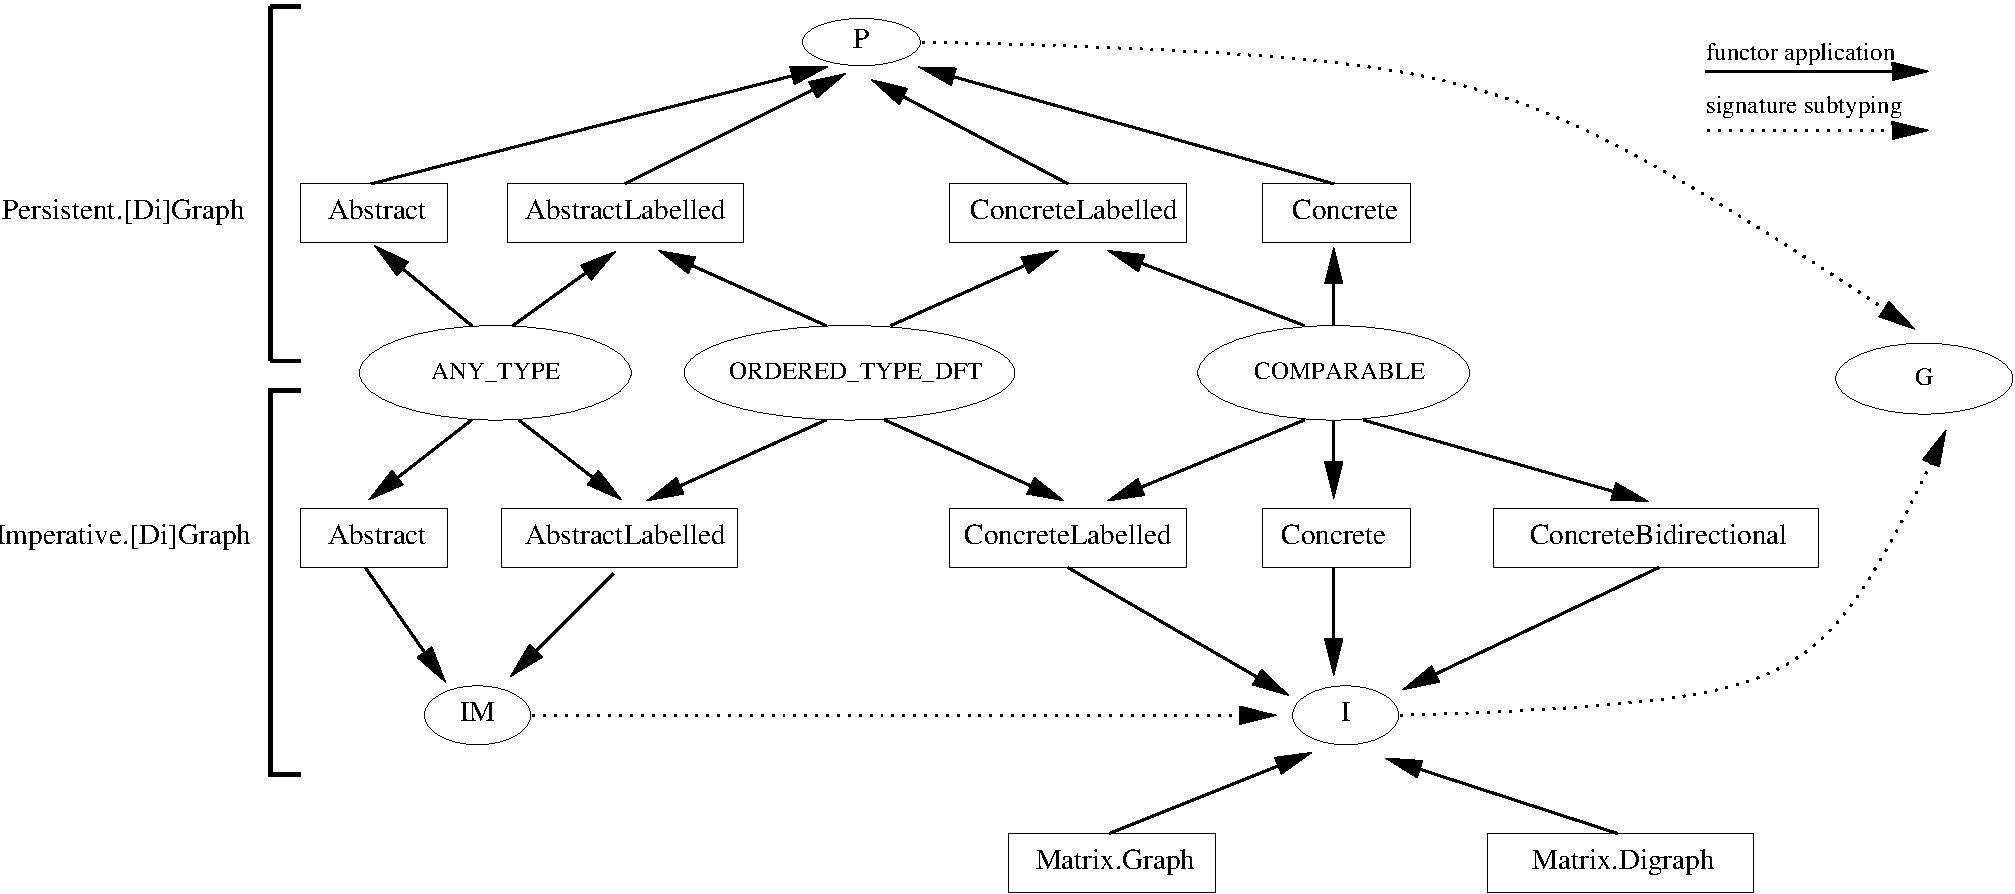
\includegraphics[width=\textwidth]{interface.pdf}    
  \caption{\ocamlgraph's data structures components}\label{fig:interfaces}
\end{figure*}

Three other implementations complete the set of graph data structures,
namely \texttt{ConcreteBidirectional} for graphs with an efficient
access to predecessors, and
\texttt{Matrix.}(\texttt{Graph},\texttt{Digraph}) for graphs
implemented as adjacency matrices.

The remaining of this section details the signatures and the modules
displayed Figure~\ref{fig:interfaces}. More precisely,
Section~\ref{interfaces} shows how the interfaces for all the
data structures are unified in order to ease the access to the library.
Then Section~\ref{codesharing} explains how the code is shared between
the various implementations.

\subsection{Interfaces}\label{interfaces}

The various graph data structures interfaces are gathered in the
module \texttt{Sig}. There are three main signatures: a common
signature \texttt{G} for all data structures, a signature \texttt{P}
for persistent data structures and a signature \texttt{I} for
imperative data structures. The common interface \texttt{G} contains
all access operations. The interfaces \texttt{P} and \texttt{I} extend
\texttt{G} by adding creation and modification operations, obviously
different for persistent and imperative data structures.

The common interface \texttt{G} introduces an abstract data type
\texttt{t} for graphs:
\begin{alltt}
module type G = sig
  type t  \hfill(* the type of graphs *)
\end{alltt}
The type of vertices is also an abstract type\footnote{The type of
  vertices is abstract in this generic interface but a particular
  implementation may declare a manifest type.}.
Since we do not know yet whether the vertices will be labeled or not,
we also introduce a type for vertices labels. (One could have
considered a polymorphic type for vertices but polymorphism does not
marry nicely with functors.) Finally, most graph algorithms require to
store vertices in data structures such as sets or dictionaries and
thus it is convenient to have the type of vertices equipped with
comparison and hashing functions. We gather all these types and
functions within a sub-module \texttt{V}:
\begin{alltt}
  module V : sig
    type t  \hfill(* the type of vertices *)
    type label  \hfill(* vertices labels *)
    val create : label -> t
    val label : t -> label
    val compare : t -> t -> int 
    val hash : t -> int 
    val equal : t -> t -> bool
  end
\end{alltt}
Introducing a sub-module has several advantages: first, it avoids
polluting the name space; second, it allows this sub-module to be
directly used as an argument of functors from \ocaml's
standard library. Yet we introduce an alias for the type
\texttt{V.t} for a greater clarity in the following:
\begin{alltt}
  type vertex = V.t
\end{alltt}
For graphs where vertices are unlabeled, we will identify the types
\texttt{V.t} and \texttt{V.label} and we will implement the operations
\texttt{V.create} and \texttt{V.label} as the identity.

Similarly, we introduce a sub-module \texttt{E} for edges. Again, we
assume that the edges may be labeled and an edge is thus built from
two vertices and a label. Finally, we equip the edges type with a
comparison function as we did for vertices.
\begin{alltt}
  module E : sig
    type t   \hfill(* the type of edges *)
    type label \hfill(* edges labels *)
    val create : vertex -> label -> vertex -> t
    val src : t -> vertex
    val dst : t -> vertex
    val label : t -> label
    val compare : t -> t -> int
  end
  type edge = E.t
\end{alltt}
For unlabeled edges, we will implement the type \texttt{E.t} as
\texttt{V.t * V.t} and we will ignore the type \texttt{E.label}
(implementing it with the \texttt{unit} type for instance).

Then we introduce a large set of test, access and iteration
functions over vertices and edges, whose meaning is immediate:
\begin{alltt}
  val is_directed : bool
  val nb_vertex : t -> int
  val out_degree : t -> vertex -> int
  val iter_vertex : (vertex -> unit) -> t -> unit
  (* ... *)
\end{alltt}
The central part of the interface is the set of functions giving
access to the graph structure. One can find for instance a function
returning the successors of a vertex as a list of vertices:
\begin{alltt}
  val succ : t -> vertex -> vertex list
  (* ... *)
\end{alltt}
In practice, however, it is more useful to iterate a given function
over the successors (or the predecessors), to avoid building a list
that would be immediately deconstructed.  This set of iterators
completes the signature \texttt{G}:
\begin{alltt}
  val iter_succ : 
    (vertex -> unit) -> t -> vertex -> unit
  val fold_succ : 
    (vertex -> 'a -> 'a) -> t -> vertex -> 'a -> 'a
  (* ... *)
end
\end{alltt}
As demonstrated in Section~\ref{algos}, implementing a graph algorithm
usually requires a small subset of these operations. Using signatures
sub-typing, any implementation of the signature \texttt{G} will also
be an adequate signature for our algorithms.

The interface \texttt{P} for persistent graphs then extends the interface
\texttt{G} with a set of creation functions:
\begin{alltt}
module type P = sig
  include G
  val empty : t
  val add_vertex : t -> vertex -> t
  val remove_vertex : t -> vertex -> t
  val add_edge : t -> vertex -> vertex -> t
  (* ... *)
end
\end{alltt}
Similarly, the interface \texttt{I} for imperative graphs extends
\texttt{G} with creation and modification functions:
\begin{alltt}
module type I = sig
  include G
  val create : unit -> t
  val copy : t -> t
  val add_vertex : t -> vertex -> unit
  val add_edge : t -> vertex -> vertex -> unit
  (* ... *)
end
\end{alltt}
One can notice the \texttt{copy} function which has no counterpart in
the interface \texttt{P}.

In Section~\ref{builder} we will show how to give a common interface
to graphs creation, whatever their persistent or imperative nature is,
in order to share code in some algorithms that need to build graphs.
But it would have been unfortunate to do it here, since the mutability
of the graph must appear clearly to the user when looking at the signature.

Finally, the module \texttt{Sig} introduces a fourth (and last)
signature for graphs, \texttt{IM}, for imperative data structures
where vertices are equipped with integers \emph{marks} which can be
modified in-place:
\begin{alltt}
module type IM = sig
  include I
  module Mark : sig
    val clear : t -> unit \hfill (* set all marks to 0 *)
    val get : vertex -> int
    val set : vertex -> int -> unit
  end
end
\end{alltt}
Such a signature is useful when one wants to provide an efficient
implementation of an algorithm based on a specific marking of the
vertices. Moreover, such marks can then be exploited by the user once the 
algorithm's run is completed, since they are exposed in the signature.
The typical example is a depth-first traversal.

One can notice that the directed nature of the graph does appear
nowhere in the signature. Only the \emph{implementations} will set
it. 

\subsection{Code Sharing}\label{codesharing}

The implementations of the various data structures for graphs are
gathered in the two modules \texttt{Persistent} and
\texttt{Imperative}. Each of these two modules is divided into two
sub-modules: \texttt{Graph} for undirected graphs and \texttt{Digraph}
for directed ones. Each of these sub-modules contains four functors,
corresponding to concrete or abstract data types\footnote{An abstract
  graph hides the representation of vertices and edges, allowing an
  optimized implementation of some operations.} with labeled or
unlabeled edges (vertices are always labeled). These functors are
parameterized by a module \texttt{V} giving the type of the vertices and,
when meaningful, by a module \texttt{E} giving the type of the edges.
For instance, the functor \texttt{Persistent.Digraph.Abstract}
implements directed persistent graphs, implemented as an abstract data
type and with no labels on edges. Its signature is the following:
\begin{alltt}
  module Abstract(V: sig type t end) : 
    Sig.P with type V.label = V.t
\end{alltt}

In the remaining of this section, we show how functors are used to
share as much code as possible among these 16 data structures. Note
the code presented here is not useful (and actually not visible) for
the user of the library.

The module \texttt{Per\_imp}, which is internal to \ocamlgraph,
gathers a few functors implementing operations that are common to
persistent and imperative graphs. Each functor has a dedicated task,
such as adding labels on edges (functor \texttt{Labelled}), makes the
graph abstract (functor \texttt{Make\_Abstract}) or adding the
operations on predecessors (functor \texttt{Pred}). Then implementing
a given graph data structure is a matter of assembling the various
functors as in a construction game and adding the few operations that
could not be factorized.

\paragraph{Abstracting the persistent or imperative nature.}
In our library, graphs are represented as dictionaries mapping each
vertex to the set of its successors (with the corresponding edge's label
if any). These dictionaries are either persistent or imperative. In
\ocaml, it results in operations with different types. Indeed, adding
a mapping into an hash table does not return any value but adding it
into a persistent map (an AVL for instance) returns a new map. 
Yet it is possible to give these persistent and imperative maps a
common signature using an explicit \texttt{'a return} type for the
returned value:
\begin{alltt}
module type HM = sig
  type 'a return 
  \hfill (* return type for [add] and [remove] *)
  type 'a t
  type key
  val add: key -> 'a -> 'a t -> 'a return
  val mem: key -> 'a t -> bool
  val find: key -> 'a t -> 'a
  (* ... *)
end
\end{alltt}
It is then possible to get a persistent implementation of \texttt{HM}
using \ocaml's \texttt{Map} module by instantiating the type
\texttt{'a return} with the type of persistent maps:
\begin{alltt}
module Make_Map(X: (* ... *) ) = struct
  include Map.Make(X)
  type 'a return = 'a t
  (* ... *)
end
\end{alltt}
Beside, it is also possible to get an imperative implementation using
\ocaml's \texttt{Hashtbl} module by instantiating the type \texttt{'a
  return} with \texttt{unit}:
\begin{alltt}
module Make_Hashtbl(X: (* ... *) ) = struct
  include Hashtbl.Make(X)
  type 'a return = unit
  let add k v h = replace h k v
  (* ... *)
end
\end{alltt}

Now, using an implementation of \texttt{HM} together with an
implementation of finite sets, it is possible to write a functor
implementing the operations which are common to all graphs:
\begin{alltt}
module Minimal(S: Set.S)(HM: HM) = struct
  let mem_vertex g v = 
    HM.mem v g
  let unsafe_add_edge g v1 v2 = 
    HM.add v1 (S.add v2 (HM.find v1 g)) g
  (* ... *)
end
\end{alltt}

\paragraph{Functors as building blocks.}
Operations over predecessors are always implemented the same way. They
are provided by the \texttt{Pred} functor:
\begin{alltt}
module Pred(S: (* ... *) ) = struct
  let fold_pred f g v = (* ... *)
  let pred g v = 
    fold_pred (fun v l -> v :: l) g v []
  (* ... *)
end
\end{alltt}
% JCF: je supprimme ceci car ce n'est pas fait ainsi dans le code
% 
% En outre, dans le cas des graphes non orient�s, les op�rations sur les
% pr�d�cesseurs peuvent �tre optimis�es en tenant compte du fait que l'ensemble
% des pr�d�cesseurs d'un sommet $s$ est �gal � l'ensemble des successeurs de $s$.
% On peut alors red�finir \texttt{Pred}:
% \begin{alltt}
% module Pred(S: (* ... *) ) = struct
%   let fold_pred = S.fold_succ
%   let pred = S.succ
%   (* ... *)
% end
% \end{alltt}
Similarly, two functors \texttt{Labeled} and \texttt{Unlabeled}
introduce all operations that depend on the presence or absence of
labels on edges, such as iterating over the edges, over the successors
of some vertex, etc.

The abstraction of a graph data structure is an operation that
encapsulates the type of vertices given by the user in some more
efficient data structure (typically a record with a unique integer).
When this is done, some operations can be optimized, such as counting
the number of vertices in the graph, since the user does not have a
direct access to the vertices anymore. The functor
\texttt{Make\_Abstract} realizes such an optimization:
\begin{alltt}
module Make_Abstract(G: Sig.G) = struct
  module I = struct
    type t = \{ edges: G.t; mutable size: int \}
    let iter_vertex f g = G.iter_vertex f g.edges
    (* ... *)
  end
  include I
  include Pred(I)
  let nb_vertex g = g.size \hfill (* optimization *)
  (* ... *)
end
\end{alltt}

Finally, it is possible to implement the concrete version of the
module \texttt{V} and the corresponding association table, given a
user data type for the vertices, using a higher-order functor:
\begin{alltt}
module ConcreteVertex
  (F: functor(X: (* ... *) ) -> 
      HM with type key = X.t)
  (V: (* ... *) ) =
struct
  module V = struct
    include V
    type label = t
    let label v = v
    let create v = v
  end
  module HM = F(V)
end
\end{alltt}

\paragraph{Assembling the blocks.}
Using all these functors, it is now possible to implement in a generic
and easy way the major part of the modules \texttt{Digraph} and
\texttt{Graph} as the following higher-order functor: 
\begin{alltt}
module Make(F: functor(X: (* ... *) ) -> 
               HM with type key = X.t) = 
struct
  module Digraph = struct
    module Concrete(V: (* ... *) ) = struct
      include ConcreteVertex(F)(V) 
        \hfill (* vertices are concrete *)
      include Unlabeled(V)(HM) 
        \hfill (* edges are unlabeled *)
      include Minimal(S)(HM) 
        \hfill (* common operations *)
    end
    module ConcreteLabelled = (* ... *)
    module Abstract = (* ... *)
    module AbstractLabelled = (* ... *)
    end
  end
  module Graph = struct (* ... *) end
end
\end{alltt}
The persistent and imperative implementations are then obtained by
applying this functor respectively to \texttt{Make\_Map} and
\texttt{Make\_Hashtbl}:
\begin{alltt}
module P = Make(Make_Map)
module I = Make(Make_Hashtbl)
\end{alltt}
Finally, to get the functors provided to the user, we simply need to
add the operations that could not be factorized:
\begin{alltt}
module Digraph = struct
  module Concrete(V: (* ... *) ) = struct
    include P.Digraph.Concrete(V) 
    let add_vertex g v1 v2 = 
      if HM.mem v g then g else add_vertex g v
    (* ... *)
  end
  (* ... *)
end
\end{alltt}

Putting all together, the code for the 19 graph data structures amounts
to 1059 lines. This is clearly small enough to be easily
maintained. In Section~\ref{bench} we will show that this code is also
quite efficient.

\section{Algorithms}\label{algos}

This section introduces the second use of functors in \ocamlgraph: the
generic programming of graph algorithms.

\subsection{Generic Programming}

As demonstrated in the previous section, our library provides many
graph data structures. Therefore, it is necessary to figure out how to
implement graph algorithms without duplicating code for each data
structure. Exactly as functors helped factorizing code in the previous
section, they provide a nice way to code the algorithms in a generic
way.

The basic idea is to code an algorithm without worrying about the
underlying graph data structure but focusing only on the required
operations over this data structure. Then the algorithm is naturally a
functor parameterized by these operations. Such operations usually
make a subset of the operations provided by \ocamlgraph's own data
structures, but some algorithms may require specific operations,
independent of the graph data structure. In such a case, they will be
provided as an additional functor parameter.

Such a ``functorization'' of algorithms has two benefits: first, it
allows to quickly add a new algorithm to the library, without code
duplication for all data structures; second, it allows the user to
apply an algorithm on its own graph data structure, which is an
original feature of \ocamlgraph\ w.r.t. other graph libraries.

\subsection{Example: Flow Algorithms}
\label{algos-flot}

We illustrate the generic implementation of algorithms in \ocamlgraph\
through two algorithms to compute the maximal flow of a
network\footnote{that is a directed graph with two distinguished
  vertices, a source and a terminal.}, namely the
Ford-Fulkerson~\cite{FF} and Goldberg~\cite{Goldberg} algorithms.
They appear as two functors with the following signatures:
\begin{alltt}
module Ford_Fulkerson 
  (G: G_FORD_FULKERSON)
  (F: FLOW with type label = G.E.label) :
sig
  val maxflow : 
    G.t -> G.V.t -> G.V.t -> (G.E.t -> F.t) * F.t
end

module Goldberg
  (G: G_GOLDBERG)
  (F: FLOW with type label = G.E.label) : 
sig
  val maxflow : 
    G.t -> G.V.t -> G.V.t -> (G.E.t -> F.t) * F.t
end
\end{alltt}
Each functor body implements a \texttt{maxflow} function expecting a
network, a source vertex and a terminal vertex, and returning a
pair \texttt{(f, delta)} where \texttt{f} maps each edge of the
network to its new flow and where \texttt{delta} is the difference
between the computed maximal flow and the initial flow of the network.

The signature of the first parameter \texttt{G} of these two functors
describes the minimal set of graph operations required for the
implementation of \texttt{maxflow}. Since the two algorithms are
different, the signatures \texttt{G\_FORD\_FULKERSON} and
\texttt{G\_GOLDBERG} are thus different. For instance, Goldberg
algorithm requires to iterates over the vertices and edges of the graph,
whereas Ford-Fulkerson algorithm only requires to iterate over the
successors and predecessors of a vertex. This appears clearly in the
signatures:
\begin{alltt}
module type G_GOLDBERG = sig
  type t
  module V : sig type t (* ... *) end
  module E : sig type t (* ... *) end
  val iter_vertex : (V.t -> unit) -> t -> unit
  val iter_edges_e : (E.t -> unit) -> t -> unit
  (* ... *)
end

module type G_FORD_FULKERSON = sig
  type t
  module V : sig type t (* ... *) end
  module E : sig type t (* ... *) end
  val iter_succ_e : 
    (E.t -> unit) -> t -> V.t -> unit
  val iter_pred_e : 
    (E.t -> unit) -> t -> V.t -> unit
end
\end{alltt}

The signature of the second parameter \texttt{F} is common to both
algorithms. It gathers all operations to manipulate the labels on edges
as flows:
\begin{alltt}
module type FLOW = sig
  type label \hfill(* type of edges labels *)
  type t \hfill(* type of flow *)
  val flow : label -> t \hfill(* initial flow *)
  val max_capacity : label -> t \hfill(* max. capacity *)
  val min_capacity : label -> t \hfill(* min. capacity *)
  val add : t -> t -> t \hfill(* addition *)
  val sub : t -> t -> t \hfill(* subtraction *)
  val zero : t \hfill (* neutral element *)
  val compare : t -> t -> int \hfill(* comparison *)
end
\end{alltt}
This signature \texttt{FLOW} is easily implemented, whatever the
data type is. For instance, a possible implementation for a graph where
edges are labeled with integers representing the maximal capacities of
edges and with an initial empty flow would be the following:
\begin{alltt}
module Flow = struct
  type label = int
  type t = int
  let max_capacity x = x
  let min_capacity _ = 0
  let flow _ = 0
  let add = (+)
  let sub = (-)
  let compare = compare
  let zero = 0
end
\end{alltt}

\subsection{Example: Graph Traversal}
\label{dfs}

We give here another example of generic programming with the classical
depth-first and breadth-first traversals. To traverse a graph, we
need very few operations. Basically, we need to iterate over the
successors of a vertex. To reach all the connected components of the
graph, we also need to iterate over all vertices. Finally, we have to
mark the visited vertices. Regarding this last point, the simplest way is
to use a hash table (when no particular assumption can be made about
the graph data structure). To build such a hash table, we simply need
the type of vertices to be equipped with suitable \texttt{hash} and
\texttt{equal} functions. Therefore, the minimal expected signature
for traversal algorithms is the following:
\begin{alltt}
module type G = sig
  type t
  module V : sig type t 
                 val hash : t -> int 
                 val equal : t -> t -> bool end
  val iter_vertex : (V.t -> unit) -> t -> unit
  val iter_succ : (V.t -> unit) -> t -> V.t -> unit
end
\end{alltt}
Then traversal algorithms can be provided with a signature like:
\begin{alltt}
module Dfs(G : G) : 
  sig val iter : (G.V.t -> unit) -> G.t -> unit end
\end{alltt}
In practice, however, several variants of each traversal are provided:
traversal of a single connected component, application of the visitor
function after the successors are visited (instead of before),
etc. The depth-first traversal functor also provides a cycle detection
function. Finally, there is a functor specialized for graphs equipped
with marks (see signature \texttt{IM} in Section~\ref{interfaces}),
since such marks can be directly used to mark the visited vertices (and
for further use by the library client).

Graph traversals are also provided as \emph{cursors},
i.e. step-by-step iterators similar to those used in object-oriented
programming~\cite{coplien92} (e.g. the \textsc{Java}
\texttt{Iterator} interface).
Such a cursor is given the following signature:
\begin{alltt}
module Dfs(G : G) : sig
  type iterator
  val start : G.t -> iterator
  val step : iterator -> iterator
  val get : iterator -> G.V.t
end 
\end{alltt}
The abstract type \texttt{iterator} represents a state of the
iterator, or equivalently a position in the ongoing iteration. We get
the starting point with the \texttt{start} function. Then we can
advance in the iteration using the \texttt{step} function and we can
obtain the currently visited vertex using the \texttt{get} function.
These two functions raise the \texttt{Exit} exception whenever the
iteration is over. There is a huge difference w.r.t. usual cursors in
imperative programming, however: the data type \texttt{iterator} is
persistent. It means that the iterator is not modified when the step
function is called, but a new iterator is returned instead. Therefore
it is easy to use such iterators in \emph{backtracking} algorithms
that may need to come back to previous positions in an
iteration~\cite{filliatre06}. 

Here is for instance a simple implementation of a $k$-coloring
algorithm based on a breadth-first traversal implemented as a
persistent cursor. We assume that the graph \texttt{g} contains
integer marks that we use to indicate the color (the value 0 meaning
that there is no assigned color yet).
\begin{alltt}
let coloring g k =
  Mark.clear g;
  let try_color v i =
    iter_succ 
      (fun w -> 
        if Mark.get w = i then raise NoColor) 
      g v;
    Mark.set v i
  in
  let rec iterate iter =
    let v = Bfs.get iter in
    for i = 1 to k do
      try try_color v i; iterate (Bfs.step iter); 
          assert false
      with NoColor -> ()
    done;
    Mark.set v 0; raise NoColor
  in
  try iterate (Bfs.start g); assert false 
  with Exit -> ()
\end{alltt}
The benefits of the persistent cursor are twofold: first, we could use
an existing traversal function without having to mix its code with the
coloring algorithm itself; second, the persistent nature of the
iterator avoids an explicit backtracking in the above code.

\subsection{Building Graphs}\label{builder}

In Section~\ref{interfaces}, we have shown that persistent and
imperative graphs have creation functions with different
signatures. However, as we have written algorithms in a generic way,
we may want to build graphs in a generic way, that is independently of
the underlying data structure. For instance, we may want to implement
graph operations (such as union, transitive closure, etc.) or to build
some classic graphs (such as the full graph with $n$ vertices, the de
Bruijn graph of order $n$, etc.) or even random graphs. In all these
cases, the persistent or imperative nature of the graph is not really
significant but the signature difference disallows genericity.

To solve this issue, we introduce a module \texttt{Builder}. It
defines a common interface for graphs building:
\begin{alltt}
module type S = sig
  module G : Sig.G
  val empty : unit -> G.t
  val copy : G.t -> G.t
  val add_vertex : G.t -> G.V.t -> G.t
  val add_edge : G.t -> G.V.t -> G.V.t -> G.t
  val add_edge_e : G.t -> G.E.t -> G.t
end
\end{alltt}
It is immediate to realize such a signature for persistent or
imperative graphs:
\begin{alltt}
module P(G : Sig.P) : S with module G = G
module I(G : Sig.I) : S with module G = G
\end{alltt}
It is important to notice that for imperative graphs the values
returned by the functions \texttt{add\_vertex},
\texttt{add\_edge} and \texttt{add\_edge\_e} are meaningless.

Therefore, it is easy to write a generic algorithm that builds
graphs. First we write a highly generic version as a functor taking a
module of signature \texttt{Builder.S} as argument:
\begin{alltt}
module Make(B : Builder.S) = struct ... end
\end{alltt}
and then we can trivially provide two variants of this functor for
both persistent and imperative graphs, with the following two lines:
\begin{alltt}
module P(G : Sig.P) = Make(Builder.P(G))
module I(G : Sig.I) = Make(Builder.I(G))
\end{alltt}
Thus the use of the module \texttt{Builder} is entirely hidden from
the user point of view.

\section{Using \ocamlgraph}\label{exemples}

This section demonstrates how to use \ocamlgraph's functors on two
typical situations: first, a direct use of \ocamlgraph's data
structures and algorithms to solve a problem; second, a more complex
situation where the user applies an \ocamlgraph's algorithm on his own
graph data structure.

\subsection{Sudoku}

This section illustrates the use of \ocamlgraph\ to solve the Sudoku
puzzle using graph coloring. This idea is to represent the Sudoku grid
as an undirected graph with $9\times 9$ vertices, each vertex being
connected to the other vertices on the same row, column or $3\times 3$
group. Then solving the Sudoku is equivalent to 9-coloring this graph.

First, we create a new graph data structure where vertices are labeled with
pairs of integers (the coordinates in the grid, as integers in the
range 0..8):
\begin{alltt}
module G = Imperative.Graph.Abstract
             (struct type t = int * int end)
\end{alltt}
We use the \texttt{Imperative} module since persistence is not
needed here, the \texttt{Graph} sub-module to indicate undirected
graphs and the \texttt{Abstract} functor both for efficiency and
simplicity. Indeed, such graphs come with integers marks on the vertices
that will be used here to store the colors.

Then we can create the graph itself:
\begin{alltt}
let g = G.create ()
\end{alltt}
This graph is initially empty. We need to create and add the 81
vertices. We could do it as simply as:
\begin{alltt}
for i = 0 to 8 do for j = 0 to 8 do 
  G.add_vertex g (G.V.create (i,j))
done done
\end{alltt}
but in order to access the vertices in the remaining of the code we
store them in a matrix:
\begin{alltt}
let vert = 
  let new_vertex i j = 
    let v = G.V.create (i, j) in 
    G.add_vertex g v; v in
  Array.init 9 (fun i -> Array.init 9 (new_vertex i))
\end{alltt}
Then we add the edges, connecting the vertices on a same row, column or group:
\begin{alltt}
for i = 0 to 8 do for j = 0 to 8 do
  for k = 0 to 8 do
    if k <> i then 
      G.add_edge g vert.(i).(j) vert.(k).(j);
    if k <> j then 
      G.add_edge g vert.(i).(j) vert.(i).(k);
  done;
  let gi = 3 * (i / 3) and gj = 3 * (j / 3) in
  for di = 0 to 2 do for dj = 0 to 2 do
    let i' = gi + di and j' = gj + dj in
    if i' <> i || j' <> j then 
      G.add_edge g vert.(i).(j) vert.(i').(j')
  done done
done done
\end{alltt}
The initial constraints in the Sudoku puzzle are set using the
\texttt{G.Mark.set} function.

To get the coloring algorithm for our graph data structure, we simply
apply the \texttt{Coloring.Mark} functor on \texttt{G}:
\begin{alltt}
module C = Coloring.Mark(G)
\end{alltt}
Finally, solving the Sudoku amounts to 9-coloring the graph \texttt{g}:
\begin{alltt}
C.coloring g 9
\end{alltt}

This code is almost as efficient as a hand-coded Sudoku solver: on the
average, a Sudoku puzzle is solved in 0.2 seconds (on a Pentium 4 2.4 GHz).

\subsection{Topological Sorting}

This section illustrates the use of one of \ocamlgraph's traversal
algorithms to perform some topological sorting on a set of files
dependencies. We assume given the following user-defined data
structure representing a file with its dependencies:
\begin{alltt}
type file = 
  \{ name : string ; mutable deps : file list \} 
\end{alltt}
In order to get the set of dependencies for a given file, we just have
to visit the underlying graph using a depth-first traversal. For that
purpose, we can use \ocamlgraph's \texttt{Graph.Traverse.Dfs}
functor (which is similar to the one presented Section~\ref{dfs}). To
do so, we need to build a 
module that implements the required graph operations.
First, we embed the \texttt{file} data type in a \texttt{Vertex} module:
\begin{alltt}
module Vertex = struct 
  type t = file 
  let compare n1 n2 = compare n1.name n2.name
  let hash n = Hashtbl.hash n.name
  let equal n1 n2 = n1.name = n2.name
end
\end{alltt}
Then viewing a list of files as a graph is easily implemented by the
following module: 
\begin{alltt}
module G = struct
  type t = file list

  module V = Vertex

  let iter_vertex = List.iter
  let fold_vertex = List.fold_right
  let iter_succ f _ v = List.iter f v.deps
  let fold_succ f _ v = List.fold_right f v.deps
end
\end{alltt}
Finally, we obtain the depth-first traversal module as a functor
instantiation: 
\begin{alltt}
module Dfs = Graph.Traverse.Dfs(G)
\end{alltt}

\section{Benchmarks}\label{bench}

Surprisingly, we could not find any standard benchmark for graph
libraries. Thus we present here the results of a little benchmark of
our own, mostly to give the reader a rough idea of \ocamlgraph efficiency.
We test four different data structures for undirected
graphs with unlabeled edges, that are either persistent (P) or
imperative (I) and with either abstract (A) or concrete (C) vertices. In
the following they are referred to as PA, PC, IA and IC, respectively.
All tests were performed on a Pentium 4 2.4 GHz.

We first test the efficiency of graph creation and mutation. 
For that purpose, we build full graphs with $V$ vertices (and thus
$E=V(V+1)/2$ edges since we include self loops). 
Then we repeatedly delete all edges and vertices in these graphs. 
Figure~\ref{fig:bench:build} displays the creation and deletion
timings in seconds up to $V=1000$ (that is half a million of edges). 
The creation speed observed is roughly 100,000 edges per second for
imperative graphs. The creation of persistent graphs is slower but
within a constant factor (less than 2). Deletion is roughly twice
faster than creation.
Regarding memory consumption, all four data structures roughly use 5
machine words (typically 20 bytes) per edge.

\begin{figure*}
  \centering\hspace*{-2em}
  \begin{tabular}{cc}
  \begin{minipage}{0.5\linewidth}
    % GNUPLOT: LaTeX picture
\setlength{\unitlength}{0.240900pt}
\ifx\plotpoint\undefined\newsavebox{\plotpoint}\fi
\sbox{\plotpoint}{\rule[-0.200pt]{0.400pt}{0.400pt}}%
\begin{picture}(1049,629)(0,0)
\sbox{\plotpoint}{\rule[-0.200pt]{0.400pt}{0.400pt}}%
\put(120.0,123.0){\rule[-0.200pt]{4.818pt}{0.400pt}}
\put(100,123){\makebox(0,0)[r]{ 0}}
\put(969.0,123.0){\rule[-0.200pt]{4.818pt}{0.400pt}}
\put(120.0,170.0){\rule[-0.200pt]{4.818pt}{0.400pt}}
\put(100,170){\makebox(0,0)[r]{ 2}}
\put(969.0,170.0){\rule[-0.200pt]{4.818pt}{0.400pt}}
\put(120.0,216.0){\rule[-0.200pt]{4.818pt}{0.400pt}}
\put(100,216){\makebox(0,0)[r]{ 4}}
\put(969.0,216.0){\rule[-0.200pt]{4.818pt}{0.400pt}}
\put(120.0,263.0){\rule[-0.200pt]{4.818pt}{0.400pt}}
\put(100,263){\makebox(0,0)[r]{ 6}}
\put(969.0,263.0){\rule[-0.200pt]{4.818pt}{0.400pt}}
\put(120.0,310.0){\rule[-0.200pt]{4.818pt}{0.400pt}}
\put(100,310){\makebox(0,0)[r]{ 8}}
\put(969.0,310.0){\rule[-0.200pt]{4.818pt}{0.400pt}}
\put(120.0,357.0){\rule[-0.200pt]{4.818pt}{0.400pt}}
\put(100,357){\makebox(0,0)[r]{ 10}}
\put(969.0,357.0){\rule[-0.200pt]{4.818pt}{0.400pt}}
\put(120.0,403.0){\rule[-0.200pt]{4.818pt}{0.400pt}}
\put(100,403){\makebox(0,0)[r]{ 12}}
\put(969.0,403.0){\rule[-0.200pt]{4.818pt}{0.400pt}}
\put(120.0,450.0){\rule[-0.200pt]{4.818pt}{0.400pt}}
\put(100,450){\makebox(0,0)[r]{ 14}}
\put(969.0,450.0){\rule[-0.200pt]{4.818pt}{0.400pt}}
\put(120.0,497.0){\rule[-0.200pt]{4.818pt}{0.400pt}}
\put(100,497){\makebox(0,0)[r]{ 16}}
\put(969.0,497.0){\rule[-0.200pt]{4.818pt}{0.400pt}}
\put(120.0,543.0){\rule[-0.200pt]{4.818pt}{0.400pt}}
\put(100,543){\makebox(0,0)[r]{ 18}}
\put(969.0,543.0){\rule[-0.200pt]{4.818pt}{0.400pt}}
\put(120.0,590.0){\rule[-0.200pt]{4.818pt}{0.400pt}}
\put(100,590){\makebox(0,0)[r]{ 20}}
\put(969.0,590.0){\rule[-0.200pt]{4.818pt}{0.400pt}}
\put(120.0,123.0){\rule[-0.200pt]{0.400pt}{4.818pt}}
\put(120,82){\makebox(0,0){ 100}}
\put(120.0,570.0){\rule[-0.200pt]{0.400pt}{4.818pt}}
\put(217.0,123.0){\rule[-0.200pt]{0.400pt}{4.818pt}}
\put(217,82){\makebox(0,0){ 200}}
\put(217.0,570.0){\rule[-0.200pt]{0.400pt}{4.818pt}}
\put(313.0,123.0){\rule[-0.200pt]{0.400pt}{4.818pt}}
\put(313,82){\makebox(0,0){ 300}}
\put(313.0,570.0){\rule[-0.200pt]{0.400pt}{4.818pt}}
\put(410.0,123.0){\rule[-0.200pt]{0.400pt}{4.818pt}}
\put(410,82){\makebox(0,0){ 400}}
\put(410.0,570.0){\rule[-0.200pt]{0.400pt}{4.818pt}}
\put(506.0,123.0){\rule[-0.200pt]{0.400pt}{4.818pt}}
\put(506,82){\makebox(0,0){ 500}}
\put(506.0,570.0){\rule[-0.200pt]{0.400pt}{4.818pt}}
\put(603.0,123.0){\rule[-0.200pt]{0.400pt}{4.818pt}}
\put(603,82){\makebox(0,0){ 600}}
\put(603.0,570.0){\rule[-0.200pt]{0.400pt}{4.818pt}}
\put(699.0,123.0){\rule[-0.200pt]{0.400pt}{4.818pt}}
\put(699,82){\makebox(0,0){ 700}}
\put(699.0,570.0){\rule[-0.200pt]{0.400pt}{4.818pt}}
\put(796.0,123.0){\rule[-0.200pt]{0.400pt}{4.818pt}}
\put(796,82){\makebox(0,0){ 800}}
\put(796.0,570.0){\rule[-0.200pt]{0.400pt}{4.818pt}}
\put(892.0,123.0){\rule[-0.200pt]{0.400pt}{4.818pt}}
\put(892,82){\makebox(0,0){ 900}}
\put(892.0,570.0){\rule[-0.200pt]{0.400pt}{4.818pt}}
\put(989.0,123.0){\rule[-0.200pt]{0.400pt}{4.818pt}}
\put(989,82){\makebox(0,0){ 1000}}
\put(989.0,570.0){\rule[-0.200pt]{0.400pt}{4.818pt}}
\put(120.0,123.0){\rule[-0.200pt]{209.342pt}{0.400pt}}
\put(989.0,123.0){\rule[-0.200pt]{0.400pt}{112.500pt}}
\put(120.0,590.0){\rule[-0.200pt]{209.342pt}{0.400pt}}
\put(120.0,123.0){\rule[-0.200pt]{0.400pt}{112.500pt}}
\put(554,21){\makebox(0,0){number of nodes $V$}}
\put(180,550){\makebox(0,0)[r]{IA}}
\put(200.0,550.0){\rule[-0.200pt]{24.090pt}{0.400pt}}
\put(120,124){\usebox{\plotpoint}}
\multiput(120.00,124.60)(14.080,0.468){5}{\rule{9.800pt}{0.113pt}}
\multiput(120.00,123.17)(76.660,4.000){2}{\rule{4.900pt}{0.400pt}}
\multiput(217.00,128.58)(4.505,0.492){19}{\rule{3.591pt}{0.118pt}}
\multiput(217.00,127.17)(88.547,11.000){2}{\rule{1.795pt}{0.400pt}}
\multiput(313.00,139.58)(2.739,0.495){33}{\rule{2.256pt}{0.119pt}}
\multiput(313.00,138.17)(92.318,18.000){2}{\rule{1.128pt}{0.400pt}}
\multiput(410.00,157.58)(1.939,0.497){47}{\rule{1.636pt}{0.120pt}}
\multiput(410.00,156.17)(92.604,25.000){2}{\rule{0.818pt}{0.400pt}}
\multiput(506.00,182.58)(1.479,0.497){63}{\rule{1.276pt}{0.120pt}}
\multiput(506.00,181.17)(94.352,33.000){2}{\rule{0.638pt}{0.400pt}}
\multiput(603.00,215.58)(2.111,0.496){43}{\rule{1.770pt}{0.120pt}}
\multiput(603.00,214.17)(92.327,23.000){2}{\rule{0.885pt}{0.400pt}}
\multiput(699.00,238.58)(1.188,0.498){79}{\rule{1.046pt}{0.120pt}}
\multiput(699.00,237.17)(94.828,41.000){2}{\rule{0.523pt}{0.400pt}}
\multiput(796.00,279.58)(0.801,0.499){117}{\rule{0.740pt}{0.120pt}}
\multiput(796.00,278.17)(94.464,60.000){2}{\rule{0.370pt}{0.400pt}}
\multiput(892.00,339.58)(1.249,0.498){75}{\rule{1.095pt}{0.120pt}}
\multiput(892.00,338.17)(94.728,39.000){2}{\rule{0.547pt}{0.400pt}}
\put(180,509){\makebox(0,0)[r]{IC}}
\multiput(200,509)(20.756,0.000){5}{\usebox{\plotpoint}}
\put(300,509){\usebox{\plotpoint}}
\put(120,124){\usebox{\plotpoint}}
\multiput(120,124)(20.685,1.706){5}{\usebox{\plotpoint}}
\multiput(217,132)(20.665,1.937){5}{\usebox{\plotpoint}}
\multiput(313,141)(20.368,3.990){5}{\usebox{\plotpoint}}
\multiput(410,160)(20.086,5.231){4}{\usebox{\plotpoint}}
\multiput(506,185)(20.572,2.757){5}{\usebox{\plotpoint}}
\multiput(603,198)(18.564,9.282){5}{\usebox{\plotpoint}}
\multiput(699,246)(18.293,9.806){6}{\usebox{\plotpoint}}
\multiput(796,298)(19.299,7.639){5}{\usebox{\plotpoint}}
\multiput(892,336)(18.135,10.096){5}{\usebox{\plotpoint}}
\put(989,390){\usebox{\plotpoint}}
\sbox{\plotpoint}{\rule[-0.400pt]{0.800pt}{0.800pt}}%
\sbox{\plotpoint}{\rule[-0.200pt]{0.400pt}{0.400pt}}%
\put(180,468){\makebox(0,0)[r]{PA}}
\sbox{\plotpoint}{\rule[-0.400pt]{0.800pt}{0.800pt}}%
\put(200.0,468.0){\rule[-0.400pt]{24.090pt}{0.800pt}}
\put(120,124){\usebox{\plotpoint}}
\multiput(120.00,125.40)(5.330,0.514){13}{\rule{7.960pt}{0.124pt}}
\multiput(120.00,122.34)(80.479,10.000){2}{\rule{3.980pt}{0.800pt}}
\multiput(217.00,135.40)(5.975,0.516){11}{\rule{8.733pt}{0.124pt}}
\multiput(217.00,132.34)(77.874,9.000){2}{\rule{4.367pt}{0.800pt}}
\multiput(313.00,144.41)(2.377,0.505){35}{\rule{3.895pt}{0.122pt}}
\multiput(313.00,141.34)(88.915,21.000){2}{\rule{1.948pt}{0.800pt}}
\multiput(410.00,165.41)(1.311,0.503){67}{\rule{2.276pt}{0.121pt}}
\multiput(410.00,162.34)(91.277,37.000){2}{\rule{1.138pt}{0.800pt}}
\multiput(506.00,202.41)(0.996,0.502){91}{\rule{1.784pt}{0.121pt}}
\multiput(506.00,199.34)(93.298,49.000){2}{\rule{0.892pt}{0.800pt}}
\multiput(603.00,251.41)(1.311,0.503){67}{\rule{2.276pt}{0.121pt}}
\multiput(603.00,248.34)(91.277,37.000){2}{\rule{1.138pt}{0.800pt}}
\multiput(699.00,288.41)(0.854,0.502){107}{\rule{1.561pt}{0.121pt}}
\multiput(699.00,285.34)(93.759,57.000){2}{\rule{0.781pt}{0.800pt}}
\multiput(796.00,345.41)(0.640,0.501){143}{\rule{1.224pt}{0.121pt}}
\multiput(796.00,342.34)(93.460,75.000){2}{\rule{0.612pt}{0.800pt}}
\multiput(892.00,420.41)(0.614,0.501){151}{\rule{1.182pt}{0.121pt}}
\multiput(892.00,417.34)(94.546,79.000){2}{\rule{0.591pt}{0.800pt}}
\sbox{\plotpoint}{\rule[-0.500pt]{1.000pt}{1.000pt}}%
\sbox{\plotpoint}{\rule[-0.200pt]{0.400pt}{0.400pt}}%
\put(180,427){\makebox(0,0)[r]{PC}}
\sbox{\plotpoint}{\rule[-0.500pt]{1.000pt}{1.000pt}}%
\multiput(200,427)(20.756,0.000){5}{\usebox{\plotpoint}}
\put(300,427){\usebox{\plotpoint}}
\put(120,125){\usebox{\plotpoint}}
\multiput(120,125)(20.598,2.548){5}{\usebox{\plotpoint}}
\multiput(217,137)(20.595,2.574){5}{\usebox{\plotpoint}}
\multiput(313,149)(19.941,5.756){5}{\usebox{\plotpoint}}
\multiput(410,177)(18.718,8.969){5}{\usebox{\plotpoint}}
\multiput(506,223)(17.652,10.918){5}{\usebox{\plotpoint}}
\multiput(603,283)(18.793,8.809){5}{\usebox{\plotpoint}}
\multiput(699,328)(15.215,14.117){7}{\usebox{\plotpoint}}
\multiput(796,418)(16.771,12.229){6}{\usebox{\plotpoint}}
\multiput(892,488)(14.377,14.970){6}{\usebox{\plotpoint}}
\put(989,589){\usebox{\plotpoint}}
\sbox{\plotpoint}{\rule[-0.200pt]{0.400pt}{0.400pt}}%
\put(120.0,123.0){\rule[-0.200pt]{209.342pt}{0.400pt}}
\put(989.0,123.0){\rule[-0.200pt]{0.400pt}{112.500pt}}
\put(120.0,590.0){\rule[-0.200pt]{209.342pt}{0.400pt}}
\put(120.0,123.0){\rule[-0.200pt]{0.400pt}{112.500pt}}
\end{picture}

  \end{minipage} &
  \begin{minipage}{0.5\linewidth}
  % GNUPLOT: LaTeX picture
\setlength{\unitlength}{0.240900pt}
\ifx\plotpoint\undefined\newsavebox{\plotpoint}\fi
\begin{picture}(1049,629)(0,0)
\sbox{\plotpoint}{\rule[-0.200pt]{0.400pt}{0.400pt}}%
\put(100.0,123.0){\rule[-0.200pt]{4.818pt}{0.400pt}}
\put(80,123){\makebox(0,0)[r]{ 0}}
\put(969.0,123.0){\rule[-0.200pt]{4.818pt}{0.400pt}}
\put(100.0,175.0){\rule[-0.200pt]{4.818pt}{0.400pt}}
\put(80,175){\makebox(0,0)[r]{ 1}}
\put(969.0,175.0){\rule[-0.200pt]{4.818pt}{0.400pt}}
\put(100.0,227.0){\rule[-0.200pt]{4.818pt}{0.400pt}}
\put(80,227){\makebox(0,0)[r]{ 2}}
\put(969.0,227.0){\rule[-0.200pt]{4.818pt}{0.400pt}}
\put(100.0,279.0){\rule[-0.200pt]{4.818pt}{0.400pt}}
\put(80,279){\makebox(0,0)[r]{ 3}}
\put(969.0,279.0){\rule[-0.200pt]{4.818pt}{0.400pt}}
\put(100.0,331.0){\rule[-0.200pt]{4.818pt}{0.400pt}}
\put(80,331){\makebox(0,0)[r]{ 4}}
\put(969.0,331.0){\rule[-0.200pt]{4.818pt}{0.400pt}}
\put(100.0,382.0){\rule[-0.200pt]{4.818pt}{0.400pt}}
\put(80,382){\makebox(0,0)[r]{ 5}}
\put(969.0,382.0){\rule[-0.200pt]{4.818pt}{0.400pt}}
\put(100.0,434.0){\rule[-0.200pt]{4.818pt}{0.400pt}}
\put(80,434){\makebox(0,0)[r]{ 6}}
\put(969.0,434.0){\rule[-0.200pt]{4.818pt}{0.400pt}}
\put(100.0,486.0){\rule[-0.200pt]{4.818pt}{0.400pt}}
\put(80,486){\makebox(0,0)[r]{ 7}}
\put(969.0,486.0){\rule[-0.200pt]{4.818pt}{0.400pt}}
\put(100.0,538.0){\rule[-0.200pt]{4.818pt}{0.400pt}}
\put(80,538){\makebox(0,0)[r]{ 8}}
\put(969.0,538.0){\rule[-0.200pt]{4.818pt}{0.400pt}}
\put(100.0,590.0){\rule[-0.200pt]{4.818pt}{0.400pt}}
\put(80,590){\makebox(0,0)[r]{ 9}}
\put(969.0,590.0){\rule[-0.200pt]{4.818pt}{0.400pt}}
\put(100.0,123.0){\rule[-0.200pt]{0.400pt}{4.818pt}}
\put(100,82){\makebox(0,0){ 100}}
\put(100.0,570.0){\rule[-0.200pt]{0.400pt}{4.818pt}}
\put(199.0,123.0){\rule[-0.200pt]{0.400pt}{4.818pt}}
\put(199,82){\makebox(0,0){ 200}}
\put(199.0,570.0){\rule[-0.200pt]{0.400pt}{4.818pt}}
\put(298.0,123.0){\rule[-0.200pt]{0.400pt}{4.818pt}}
\put(298,82){\makebox(0,0){ 300}}
\put(298.0,570.0){\rule[-0.200pt]{0.400pt}{4.818pt}}
\put(396.0,123.0){\rule[-0.200pt]{0.400pt}{4.818pt}}
\put(396,82){\makebox(0,0){ 400}}
\put(396.0,570.0){\rule[-0.200pt]{0.400pt}{4.818pt}}
\put(495.0,123.0){\rule[-0.200pt]{0.400pt}{4.818pt}}
\put(495,82){\makebox(0,0){ 500}}
\put(495.0,570.0){\rule[-0.200pt]{0.400pt}{4.818pt}}
\put(594.0,123.0){\rule[-0.200pt]{0.400pt}{4.818pt}}
\put(594,82){\makebox(0,0){ 600}}
\put(594.0,570.0){\rule[-0.200pt]{0.400pt}{4.818pt}}
\put(693.0,123.0){\rule[-0.200pt]{0.400pt}{4.818pt}}
\put(693,82){\makebox(0,0){ 700}}
\put(693.0,570.0){\rule[-0.200pt]{0.400pt}{4.818pt}}
\put(791.0,123.0){\rule[-0.200pt]{0.400pt}{4.818pt}}
\put(791,82){\makebox(0,0){ 800}}
\put(791.0,570.0){\rule[-0.200pt]{0.400pt}{4.818pt}}
\put(890.0,123.0){\rule[-0.200pt]{0.400pt}{4.818pt}}
\put(890,82){\makebox(0,0){ 900}}
\put(890.0,570.0){\rule[-0.200pt]{0.400pt}{4.818pt}}
\put(989.0,123.0){\rule[-0.200pt]{0.400pt}{4.818pt}}
\put(989,82){\makebox(0,0){ 1000}}
\put(989.0,570.0){\rule[-0.200pt]{0.400pt}{4.818pt}}
\put(100.0,123.0){\rule[-0.200pt]{214.160pt}{0.400pt}}
\put(989.0,123.0){\rule[-0.200pt]{0.400pt}{112.500pt}}
\put(100.0,590.0){\rule[-0.200pt]{214.160pt}{0.400pt}}
\put(100.0,123.0){\rule[-0.200pt]{0.400pt}{112.500pt}}
\put(544,21){\makebox(0,0){number of nodes $V$}}
\put(160,550){\makebox(0,0)[r]{IA}}
\put(180.0,550.0){\rule[-0.200pt]{24.090pt}{0.400pt}}
\put(100,124){\usebox{\plotpoint}}
\multiput(100.00,124.61)(21.895,0.447){3}{\rule{13.300pt}{0.108pt}}
\multiput(100.00,123.17)(71.395,3.000){2}{\rule{6.650pt}{0.400pt}}
\multiput(199.00,127.59)(8.898,0.482){9}{\rule{6.700pt}{0.116pt}}
\multiput(199.00,126.17)(85.094,6.000){2}{\rule{3.350pt}{0.400pt}}
\multiput(298.00,133.58)(4.600,0.492){19}{\rule{3.664pt}{0.118pt}}
\multiput(298.00,132.17)(90.396,11.000){2}{\rule{1.832pt}{0.400pt}}
\multiput(396.00,144.58)(2.964,0.495){31}{\rule{2.429pt}{0.119pt}}
\multiput(396.00,143.17)(93.958,17.000){2}{\rule{1.215pt}{0.400pt}}
\multiput(495.00,161.58)(3.370,0.494){27}{\rule{2.740pt}{0.119pt}}
\multiput(495.00,160.17)(93.313,15.000){2}{\rule{1.370pt}{0.400pt}}
\multiput(594.00,176.58)(0.739,0.499){131}{\rule{0.691pt}{0.120pt}}
\multiput(594.00,175.17)(97.566,67.000){2}{\rule{0.346pt}{0.400pt}}
\multiput(693.00,241.92)(3.867,-0.493){23}{\rule{3.115pt}{0.119pt}}
\multiput(693.00,242.17)(91.534,-13.000){2}{\rule{1.558pt}{0.400pt}}
\multiput(791.58,230.00)(0.499,0.576){195}{\rule{0.120pt}{0.561pt}}
\multiput(790.17,230.00)(99.000,112.836){2}{\rule{0.400pt}{0.280pt}}
\multiput(890.00,344.58)(1.156,0.498){83}{\rule{1.021pt}{0.120pt}}
\multiput(890.00,343.17)(96.881,43.000){2}{\rule{0.510pt}{0.400pt}}
\put(160,509){\makebox(0,0)[r]{IC}}
\multiput(180,509)(20.756,0.000){5}{\usebox{\plotpoint}}
\put(280,509){\usebox{\plotpoint}}
\put(100,124){\usebox{\plotpoint}}
\multiput(100,124)(20.739,0.838){5}{\usebox{\plotpoint}}
\multiput(199,128)(20.717,1.256){5}{\usebox{\plotpoint}}
\multiput(298,134)(20.602,2.523){5}{\usebox{\plotpoint}}
\multiput(396,146)(20.754,0.210){5}{\usebox{\plotpoint}}
\multiput(495,147)(17.350,11.391){5}{\usebox{\plotpoint}}
\multiput(594,212)(20.751,-0.419){5}{\usebox{\plotpoint}}
\multiput(693,210)(15.918,13.319){6}{\usebox{\plotpoint}}
\multiput(791,292)(18.750,8.901){5}{\usebox{\plotpoint}}
\multiput(890,339)(17.028,11.868){6}{\usebox{\plotpoint}}
\put(989,408){\usebox{\plotpoint}}
\sbox{\plotpoint}{\rule[-0.400pt]{0.800pt}{0.800pt}}%
\sbox{\plotpoint}{\rule[-0.200pt]{0.400pt}{0.400pt}}%
\put(160,468){\makebox(0,0)[r]{PA}}
\sbox{\plotpoint}{\rule[-0.400pt]{0.800pt}{0.800pt}}%
\put(180.0,468.0){\rule[-0.400pt]{24.090pt}{0.800pt}}
\put(100,125){\usebox{\plotpoint}}
\multiput(100.00,126.40)(8.534,0.526){7}{\rule{11.514pt}{0.127pt}}
\multiput(100.00,123.34)(75.102,7.000){2}{\rule{5.757pt}{0.800pt}}
\multiput(199.00,133.41)(3.032,0.507){27}{\rule{4.859pt}{0.122pt}}
\multiput(199.00,130.34)(88.915,17.000){2}{\rule{2.429pt}{0.800pt}}
\multiput(298.00,150.41)(4.378,0.511){17}{\rule{6.733pt}{0.123pt}}
\multiput(298.00,147.34)(84.025,12.000){2}{\rule{3.367pt}{0.800pt}}
\multiput(396.00,162.41)(1.801,0.504){49}{\rule{3.029pt}{0.121pt}}
\multiput(396.00,159.34)(92.714,28.000){2}{\rule{1.514pt}{0.800pt}}
\multiput(495.00,190.41)(0.828,0.502){113}{\rule{1.520pt}{0.121pt}}
\multiput(495.00,187.34)(95.845,60.000){2}{\rule{0.760pt}{0.800pt}}
\multiput(594.00,250.41)(1.084,0.502){85}{\rule{1.922pt}{0.121pt}}
\multiput(594.00,247.34)(95.011,46.000){2}{\rule{0.961pt}{0.800pt}}
\multiput(693.00,296.41)(0.819,0.502){113}{\rule{1.507pt}{0.121pt}}
\multiput(693.00,293.34)(94.873,60.000){2}{\rule{0.753pt}{0.800pt}}
\multiput(791.00,356.41)(0.688,0.501){137}{\rule{1.300pt}{0.121pt}}
\multiput(791.00,353.34)(96.302,72.000){2}{\rule{0.650pt}{0.800pt}}
\multiput(890.00,428.41)(0.669,0.501){141}{\rule{1.270pt}{0.121pt}}
\multiput(890.00,425.34)(96.363,74.000){2}{\rule{0.635pt}{0.800pt}}
\sbox{\plotpoint}{\rule[-0.500pt]{1.000pt}{1.000pt}}%
\sbox{\plotpoint}{\rule[-0.200pt]{0.400pt}{0.400pt}}%
\put(160,427){\makebox(0,0)[r]{PC}}
\sbox{\plotpoint}{\rule[-0.500pt]{1.000pt}{1.000pt}}%
\multiput(180,427)(20.756,0.000){5}{\usebox{\plotpoint}}
\put(280,427){\usebox{\plotpoint}}
\put(100,125){\usebox{\plotpoint}}
\multiput(100,125)(20.704,1.464){5}{\usebox{\plotpoint}}
\multiput(199,132)(20.171,4.890){5}{\usebox{\plotpoint}}
\multiput(298,156)(20.414,3.750){5}{\usebox{\plotpoint}}
\multiput(396,174)(19.569,6.918){5}{\usebox{\plotpoint}}
\multiput(495,209)(17.350,11.391){6}{\usebox{\plotpoint}}
\multiput(594,274)(20.261,4.503){5}{\usebox{\plotpoint}}
\multiput(693,296)(13.599,15.680){7}{\usebox{\plotpoint}}
\multiput(791,409)(15.435,13.876){6}{\usebox{\plotpoint}}
\multiput(890,498)(15.984,13.240){6}{\usebox{\plotpoint}}
\put(989,580){\usebox{\plotpoint}}
\sbox{\plotpoint}{\rule[-0.200pt]{0.400pt}{0.400pt}}%
\put(100.0,123.0){\rule[-0.200pt]{214.160pt}{0.400pt}}
\put(989.0,123.0){\rule[-0.200pt]{0.400pt}{112.500pt}}
\put(100.0,590.0){\rule[-0.200pt]{214.160pt}{0.400pt}}
\put(100.0,123.0){\rule[-0.200pt]{0.400pt}{112.500pt}}
\end{picture}

  \end{minipage}
  \end{tabular}
  \caption{Benchmarking creation (left) and deletion (right)}
  \label{fig:bench:build}
\end{figure*}

Our second benchmark consists in building graphs corresponding to 2D
mazes, using a percolation algorithm, and then traversing them using
depth-first and breadth-first traversals. Given an integer $N$, we
build a graph with $V=N^2$ vertices and $E=V-1$
edges. Figure~\ref{fig:bench:maze} displays the timings in seconds for various
values of $N$ up to 600 (i.e. 360,000 vertices). The observed speed is
between 500,000 and 1 million traversed edges per second.

% on enleve Dijkstra parce que le resultat est bizarre
% % GNUPLOT: LaTeX picture
\setlength{\unitlength}{0.240900pt}
\ifx\plotpoint\undefined\newsavebox{\plotpoint}\fi
\begin{picture}(1049,629)(0,0)
\sbox{\plotpoint}{\rule[-0.200pt]{0.400pt}{0.400pt}}%
\put(140.0,123.0){\rule[-0.200pt]{4.818pt}{0.400pt}}
\put(120,123){\makebox(0,0)[r]{ 0}}
\put(969.0,123.0){\rule[-0.200pt]{4.818pt}{0.400pt}}
\put(140.0,216.0){\rule[-0.200pt]{4.818pt}{0.400pt}}
\put(120,216){\makebox(0,0)[r]{ 0.5}}
\put(969.0,216.0){\rule[-0.200pt]{4.818pt}{0.400pt}}
\put(140.0,310.0){\rule[-0.200pt]{4.818pt}{0.400pt}}
\put(120,310){\makebox(0,0)[r]{ 1}}
\put(969.0,310.0){\rule[-0.200pt]{4.818pt}{0.400pt}}
\put(140.0,403.0){\rule[-0.200pt]{4.818pt}{0.400pt}}
\put(120,403){\makebox(0,0)[r]{ 1.5}}
\put(969.0,403.0){\rule[-0.200pt]{4.818pt}{0.400pt}}
\put(140.0,497.0){\rule[-0.200pt]{4.818pt}{0.400pt}}
\put(120,497){\makebox(0,0)[r]{ 2}}
\put(969.0,497.0){\rule[-0.200pt]{4.818pt}{0.400pt}}
\put(140.0,590.0){\rule[-0.200pt]{4.818pt}{0.400pt}}
\put(120,590){\makebox(0,0)[r]{ 2.5}}
\put(969.0,590.0){\rule[-0.200pt]{4.818pt}{0.400pt}}
\put(140.0,123.0){\rule[-0.200pt]{0.400pt}{4.818pt}}
\put(140,82){\makebox(0,0){ 0}}
\put(140.0,570.0){\rule[-0.200pt]{0.400pt}{4.818pt}}
\put(282.0,123.0){\rule[-0.200pt]{0.400pt}{4.818pt}}
\put(282,82){\makebox(0,0){ 100}}
\put(282.0,570.0){\rule[-0.200pt]{0.400pt}{4.818pt}}
\put(423.0,123.0){\rule[-0.200pt]{0.400pt}{4.818pt}}
\put(423,82){\makebox(0,0){ 200}}
\put(423.0,570.0){\rule[-0.200pt]{0.400pt}{4.818pt}}
\put(565.0,123.0){\rule[-0.200pt]{0.400pt}{4.818pt}}
\put(565,82){\makebox(0,0){ 300}}
\put(565.0,570.0){\rule[-0.200pt]{0.400pt}{4.818pt}}
\put(706.0,123.0){\rule[-0.200pt]{0.400pt}{4.818pt}}
\put(706,82){\makebox(0,0){ 400}}
\put(706.0,570.0){\rule[-0.200pt]{0.400pt}{4.818pt}}
\put(848.0,123.0){\rule[-0.200pt]{0.400pt}{4.818pt}}
\put(848,82){\makebox(0,0){ 500}}
\put(848.0,570.0){\rule[-0.200pt]{0.400pt}{4.818pt}}
\put(989.0,123.0){\rule[-0.200pt]{0.400pt}{4.818pt}}
\put(989,82){\makebox(0,0){ 600}}
\put(989.0,570.0){\rule[-0.200pt]{0.400pt}{4.818pt}}
\put(140.0,123.0){\rule[-0.200pt]{204.524pt}{0.400pt}}
\put(989.0,123.0){\rule[-0.200pt]{0.400pt}{112.500pt}}
\put(140.0,590.0){\rule[-0.200pt]{204.524pt}{0.400pt}}
\put(140.0,123.0){\rule[-0.200pt]{0.400pt}{112.500pt}}
\put(564,21){\makebox(0,0){maze width $N$}}
\put(200,550){\makebox(0,0)[r]{IA}}
\put(220.0,550.0){\rule[-0.200pt]{24.090pt}{0.400pt}}
\put(225,125){\usebox{\plotpoint}}
\multiput(225.00,125.59)(9.393,0.477){7}{\rule{6.900pt}{0.115pt}}
\multiput(225.00,124.17)(70.679,5.000){2}{\rule{3.450pt}{0.400pt}}
\multiput(310.00,130.58)(3.641,0.492){21}{\rule{2.933pt}{0.119pt}}
\multiput(310.00,129.17)(78.912,12.000){2}{\rule{1.467pt}{0.400pt}}
\multiput(395.00,142.58)(2.706,0.494){29}{\rule{2.225pt}{0.119pt}}
\multiput(395.00,141.17)(80.382,16.000){2}{\rule{1.113pt}{0.400pt}}
\multiput(480.00,158.58)(2.543,0.495){31}{\rule{2.100pt}{0.119pt}}
\multiput(480.00,157.17)(80.641,17.000){2}{\rule{1.050pt}{0.400pt}}
\multiput(565.00,175.58)(2.513,0.495){31}{\rule{2.076pt}{0.119pt}}
\multiput(565.00,174.17)(79.690,17.000){2}{\rule{1.038pt}{0.400pt}}
\multiput(649.00,192.58)(0.760,0.499){109}{\rule{0.707pt}{0.120pt}}
\multiput(649.00,191.17)(83.532,56.000){2}{\rule{0.354pt}{0.400pt}}
\multiput(734.00,248.58)(2.543,0.495){31}{\rule{2.100pt}{0.119pt}}
\multiput(734.00,247.17)(80.641,17.000){2}{\rule{1.050pt}{0.400pt}}
\multiput(819.58,265.00)(0.499,0.647){167}{\rule{0.120pt}{0.618pt}}
\multiput(818.17,265.00)(85.000,108.718){2}{\rule{0.400pt}{0.309pt}}
\multiput(904.58,372.28)(0.499,-0.694){167}{\rule{0.120pt}{0.655pt}}
\multiput(903.17,373.64)(85.000,-116.640){2}{\rule{0.400pt}{0.328pt}}
\put(200,509){\makebox(0,0)[r]{IC}}
\multiput(220,509)(20.756,0.000){5}{\usebox{\plotpoint}}
\put(320,509){\usebox{\plotpoint}}
\put(225,125){\usebox{\plotpoint}}
\multiput(225,125)(20.584,2.664){5}{\usebox{\plotpoint}}
\multiput(310,136)(20.640,2.185){4}{\usebox{\plotpoint}}
\multiput(395,145)(20.256,4.528){4}{\usebox{\plotpoint}}
\multiput(480,164)(19.848,6.071){4}{\usebox{\plotpoint}}
\multiput(565,190)(19.239,7.787){5}{\usebox{\plotpoint}}
\multiput(649,224)(15.563,13.732){5}{\usebox{\plotpoint}}
\multiput(734,299)(18.865,8.656){5}{\usebox{\plotpoint}}
\multiput(819,338)(10.885,17.672){7}{\usebox{\plotpoint}}
\multiput(904,476)(8.985,-18.710){10}{\usebox{\plotpoint}}
\put(989,299){\usebox{\plotpoint}}
\sbox{\plotpoint}{\rule[-0.400pt]{0.800pt}{0.800pt}}%
\sbox{\plotpoint}{\rule[-0.200pt]{0.400pt}{0.400pt}}%
\put(200,468){\makebox(0,0)[r]{PA}}
\sbox{\plotpoint}{\rule[-0.400pt]{0.800pt}{0.800pt}}%
\put(220.0,468.0){\rule[-0.400pt]{24.090pt}{0.800pt}}
\put(225,127){\usebox{\plotpoint}}
\multiput(225.00,128.38)(13.857,0.560){3}{\rule{13.800pt}{0.135pt}}
\multiput(225.00,125.34)(56.357,5.000){2}{\rule{6.900pt}{0.800pt}}
\multiput(310.00,133.41)(3.790,0.511){17}{\rule{5.867pt}{0.123pt}}
\multiput(310.00,130.34)(72.823,12.000){2}{\rule{2.933pt}{0.800pt}}
\multiput(395.00,145.41)(2.772,0.507){25}{\rule{4.450pt}{0.122pt}}
\multiput(395.00,142.34)(75.764,16.000){2}{\rule{2.225pt}{0.800pt}}
\multiput(480.00,161.41)(2.599,0.507){27}{\rule{4.200pt}{0.122pt}}
\multiput(480.00,158.34)(76.283,17.000){2}{\rule{2.100pt}{0.800pt}}
\multiput(565.00,178.41)(1.421,0.503){53}{\rule{2.440pt}{0.121pt}}
\multiput(565.00,175.34)(78.936,30.000){2}{\rule{1.220pt}{0.800pt}}
\multiput(649.00,208.41)(0.909,0.502){87}{\rule{1.647pt}{0.121pt}}
\multiput(649.00,205.34)(81.582,47.000){2}{\rule{0.823pt}{0.800pt}}
\multiput(734.00,255.41)(0.710,0.502){113}{\rule{1.333pt}{0.121pt}}
\multiput(734.00,252.34)(82.233,60.000){2}{\rule{0.667pt}{0.800pt}}
\multiput(820.41,314.00)(0.501,0.600){163}{\rule{0.121pt}{1.160pt}}
\multiput(817.34,314.00)(85.000,99.592){2}{\rule{0.800pt}{0.580pt}}
\multiput(905.41,410.87)(0.501,-0.647){163}{\rule{0.121pt}{1.235pt}}
\multiput(902.34,413.44)(85.000,-107.436){2}{\rule{0.800pt}{0.618pt}}
\sbox{\plotpoint}{\rule[-0.500pt]{1.000pt}{1.000pt}}%
\sbox{\plotpoint}{\rule[-0.200pt]{0.400pt}{0.400pt}}%
\put(200,427){\makebox(0,0)[r]{PC}}
\sbox{\plotpoint}{\rule[-0.500pt]{1.000pt}{1.000pt}}%
\multiput(220,427)(20.756,0.000){5}{\usebox{\plotpoint}}
\put(320,427){\usebox{\plotpoint}}
\put(225,127){\usebox{\plotpoint}}
\multiput(225,127)(20.640,2.185){5}{\usebox{\plotpoint}}
\multiput(310,136)(20.352,4.070){4}{\usebox{\plotpoint}}
\multiput(395,153)(19.713,6.494){4}{\usebox{\plotpoint}}
\multiput(480,181)(19.713,6.494){4}{\usebox{\plotpoint}}
\multiput(565,209)(20.078,5.259){5}{\usebox{\plotpoint}}
\multiput(649,231)(15.746,13.523){5}{\usebox{\plotpoint}}
\multiput(734,304)(17.144,11.699){5}{\usebox{\plotpoint}}
\multiput(819,362)(9.690,18.355){9}{\usebox{\plotpoint}}
\multiput(904,523)(8.823,-18.787){9}{\usebox{\plotpoint}}
\put(989,342){\usebox{\plotpoint}}
\sbox{\plotpoint}{\rule[-0.200pt]{0.400pt}{0.400pt}}%
\put(140.0,123.0){\rule[-0.200pt]{204.524pt}{0.400pt}}
\put(989.0,123.0){\rule[-0.200pt]{0.400pt}{112.500pt}}
\put(140.0,590.0){\rule[-0.200pt]{204.524pt}{0.400pt}}
\put(140.0,123.0){\rule[-0.200pt]{0.400pt}{112.500pt}}
\end{picture}


\begin{figure*}
  \centering\hspace*{-2em}
  \begin{tabular}{cc}
  \begin{minipage}{0.5\linewidth}
% GNUPLOT: LaTeX picture
\setlength{\unitlength}{0.240900pt}
\ifx\plotpoint\undefined\newsavebox{\plotpoint}\fi
\begin{picture}(1049,629)(0,0)
\sbox{\plotpoint}{\rule[-0.200pt]{0.400pt}{0.400pt}}%
\put(140.0,123.0){\rule[-0.200pt]{4.818pt}{0.400pt}}
\put(120,123){\makebox(0,0)[r]{ 0}}
\put(969.0,123.0){\rule[-0.200pt]{4.818pt}{0.400pt}}
\put(140.0,201.0){\rule[-0.200pt]{4.818pt}{0.400pt}}
\put(120,201){\makebox(0,0)[r]{ 0.5}}
\put(969.0,201.0){\rule[-0.200pt]{4.818pt}{0.400pt}}
\put(140.0,279.0){\rule[-0.200pt]{4.818pt}{0.400pt}}
\put(120,279){\makebox(0,0)[r]{ 1}}
\put(969.0,279.0){\rule[-0.200pt]{4.818pt}{0.400pt}}
\put(140.0,356.0){\rule[-0.200pt]{4.818pt}{0.400pt}}
\put(120,356){\makebox(0,0)[r]{ 1.5}}
\put(969.0,356.0){\rule[-0.200pt]{4.818pt}{0.400pt}}
\put(140.0,434.0){\rule[-0.200pt]{4.818pt}{0.400pt}}
\put(120,434){\makebox(0,0)[r]{ 2}}
\put(969.0,434.0){\rule[-0.200pt]{4.818pt}{0.400pt}}
\put(140.0,512.0){\rule[-0.200pt]{4.818pt}{0.400pt}}
\put(120,512){\makebox(0,0)[r]{ 2.5}}
\put(969.0,512.0){\rule[-0.200pt]{4.818pt}{0.400pt}}
\put(140.0,590.0){\rule[-0.200pt]{4.818pt}{0.400pt}}
\put(120,590){\makebox(0,0)[r]{ 3}}
\put(969.0,590.0){\rule[-0.200pt]{4.818pt}{0.400pt}}
\put(140.0,123.0){\rule[-0.200pt]{0.400pt}{4.818pt}}
\put(140,82){\makebox(0,0){ 0}}
\put(140.0,570.0){\rule[-0.200pt]{0.400pt}{4.818pt}}
\put(282.0,123.0){\rule[-0.200pt]{0.400pt}{4.818pt}}
\put(282,82){\makebox(0,0){ 100}}
\put(282.0,570.0){\rule[-0.200pt]{0.400pt}{4.818pt}}
\put(423.0,123.0){\rule[-0.200pt]{0.400pt}{4.818pt}}
\put(423,82){\makebox(0,0){ 200}}
\put(423.0,570.0){\rule[-0.200pt]{0.400pt}{4.818pt}}
\put(565.0,123.0){\rule[-0.200pt]{0.400pt}{4.818pt}}
\put(565,82){\makebox(0,0){ 300}}
\put(565.0,570.0){\rule[-0.200pt]{0.400pt}{4.818pt}}
\put(706.0,123.0){\rule[-0.200pt]{0.400pt}{4.818pt}}
\put(706,82){\makebox(0,0){ 400}}
\put(706.0,570.0){\rule[-0.200pt]{0.400pt}{4.818pt}}
\put(848.0,123.0){\rule[-0.200pt]{0.400pt}{4.818pt}}
\put(848,82){\makebox(0,0){ 500}}
\put(848.0,570.0){\rule[-0.200pt]{0.400pt}{4.818pt}}
\put(989.0,123.0){\rule[-0.200pt]{0.400pt}{4.818pt}}
\put(989,82){\makebox(0,0){ 600}}
\put(989.0,570.0){\rule[-0.200pt]{0.400pt}{4.818pt}}
\put(140.0,123.0){\rule[-0.200pt]{204.524pt}{0.400pt}}
\put(989.0,123.0){\rule[-0.200pt]{0.400pt}{112.500pt}}
\put(140.0,590.0){\rule[-0.200pt]{204.524pt}{0.400pt}}
\put(140.0,123.0){\rule[-0.200pt]{0.400pt}{112.500pt}}
\put(564,21){\makebox(0,0){maze width $N$}}
\put(200,550){\makebox(0,0)[r]{IA}}
\put(220.0,550.0){\rule[-0.200pt]{24.090pt}{0.400pt}}
\put(225,125){\usebox{\plotpoint}}
\multiput(225.00,125.61)(18.770,0.447){3}{\rule{11.433pt}{0.108pt}}
\multiput(225.00,124.17)(61.270,3.000){2}{\rule{5.717pt}{0.400pt}}
\multiput(310.00,128.60)(12.325,0.468){5}{\rule{8.600pt}{0.113pt}}
\multiput(310.00,127.17)(67.150,4.000){2}{\rule{4.300pt}{0.400pt}}
\multiput(395.00,132.59)(5.579,0.488){13}{\rule{4.350pt}{0.117pt}}
\multiput(395.00,131.17)(75.971,8.000){2}{\rule{2.175pt}{0.400pt}}
\multiput(480.00,140.59)(4.922,0.489){15}{\rule{3.878pt}{0.118pt}}
\multiput(480.00,139.17)(76.951,9.000){2}{\rule{1.939pt}{0.400pt}}
\multiput(565.00,149.58)(3.312,0.493){23}{\rule{2.685pt}{0.119pt}}
\multiput(565.00,148.17)(78.428,13.000){2}{\rule{1.342pt}{0.400pt}}
\multiput(649.00,162.58)(0.947,0.498){87}{\rule{0.856pt}{0.120pt}}
\multiput(649.00,161.17)(83.224,45.000){2}{\rule{0.428pt}{0.400pt}}
\multiput(734.00,207.59)(7.633,0.482){9}{\rule{5.767pt}{0.116pt}}
\multiput(734.00,206.17)(73.031,6.000){2}{\rule{2.883pt}{0.400pt}}
\multiput(819.00,213.58)(0.852,0.498){97}{\rule{0.780pt}{0.120pt}}
\multiput(819.00,212.17)(83.381,50.000){2}{\rule{0.390pt}{0.400pt}}
\multiput(904.00,263.58)(0.582,0.499){143}{\rule{0.566pt}{0.120pt}}
\multiput(904.00,262.17)(83.826,73.000){2}{\rule{0.283pt}{0.400pt}}
\put(200,509){\makebox(0,0)[r]{IC}}
\multiput(220,509)(20.756,0.000){5}{\usebox{\plotpoint}}
\put(320,509){\usebox{\plotpoint}}
\put(225,134){\usebox{\plotpoint}}
\multiput(225,134)(20.754,0.244){5}{\usebox{\plotpoint}}
\multiput(310,135)(20.720,1.219){4}{\usebox{\plotpoint}}
\multiput(395,140)(20.352,4.070){4}{\usebox{\plotpoint}}
\multiput(480,157)(19.782,6.284){4}{\usebox{\plotpoint}}
\multiput(565,184)(19.472,7.186){4}{\usebox{\plotpoint}}
\multiput(649,215)(16.207,12.966){6}{\usebox{\plotpoint}}
\multiput(734,283)(18.343,9.711){4}{\usebox{\plotpoint}}
\multiput(819,328)(15.026,14.319){6}{\usebox{\plotpoint}}
\multiput(904,409)(18.608,9.194){5}{\usebox{\plotpoint}}
\put(989,451){\usebox{\plotpoint}}
\sbox{\plotpoint}{\rule[-0.400pt]{0.800pt}{0.800pt}}%
\sbox{\plotpoint}{\rule[-0.200pt]{0.400pt}{0.400pt}}%
\put(200,468){\makebox(0,0)[r]{PA}}
\sbox{\plotpoint}{\rule[-0.400pt]{0.800pt}{0.800pt}}%
\put(220.0,468.0){\rule[-0.400pt]{24.090pt}{0.800pt}}
\put(225,128){\usebox{\plotpoint}}
\put(225,126.84){\rule{20.476pt}{0.800pt}}
\multiput(225.00,126.34)(42.500,1.000){2}{\rule{10.238pt}{0.800pt}}
\multiput(310.00,130.40)(6.111,0.520){9}{\rule{8.700pt}{0.125pt}}
\multiput(310.00,127.34)(66.943,8.000){2}{\rule{4.350pt}{0.800pt}}
\multiput(395.00,138.40)(4.179,0.512){15}{\rule{6.382pt}{0.123pt}}
\multiput(395.00,135.34)(71.754,11.000){2}{\rule{3.191pt}{0.800pt}}
\multiput(480.00,149.41)(3.790,0.511){17}{\rule{5.867pt}{0.123pt}}
\multiput(480.00,146.34)(72.823,12.000){2}{\rule{2.933pt}{0.800pt}}
\multiput(565.00,161.41)(1.288,0.503){59}{\rule{2.236pt}{0.121pt}}
\multiput(565.00,158.34)(79.358,33.000){2}{\rule{1.118pt}{0.800pt}}
\multiput(649.00,194.41)(0.972,0.502){81}{\rule{1.745pt}{0.121pt}}
\multiput(649.00,191.34)(81.377,44.000){2}{\rule{0.873pt}{0.800pt}}
\multiput(734.00,238.41)(2.446,0.506){29}{\rule{3.978pt}{0.122pt}}
\multiput(734.00,235.34)(76.744,18.000){2}{\rule{1.989pt}{0.800pt}}
\multiput(819.00,256.41)(0.761,0.502){105}{\rule{1.414pt}{0.121pt}}
\multiput(819.00,253.34)(82.065,56.000){2}{\rule{0.707pt}{0.800pt}}
\multiput(904.00,312.41)(0.761,0.502){105}{\rule{1.414pt}{0.121pt}}
\multiput(904.00,309.34)(82.065,56.000){2}{\rule{0.707pt}{0.800pt}}
\sbox{\plotpoint}{\rule[-0.500pt]{1.000pt}{1.000pt}}%
\sbox{\plotpoint}{\rule[-0.200pt]{0.400pt}{0.400pt}}%
\put(200,427){\makebox(0,0)[r]{PC}}
\sbox{\plotpoint}{\rule[-0.500pt]{1.000pt}{1.000pt}}%
\multiput(220,427)(20.756,0.000){5}{\usebox{\plotpoint}}
\put(320,427){\usebox{\plotpoint}}
\put(225,128){\usebox{\plotpoint}}
\multiput(225,128)(20.685,1.704){5}{\usebox{\plotpoint}}
\multiput(310,135)(20.480,3.373){4}{\usebox{\plotpoint}}
\multiput(395,149)(19.912,5.857){4}{\usebox{\plotpoint}}
\multiput(480,174)(19.192,7.903){4}{\usebox{\plotpoint}}
\multiput(565,209)(18.739,8.923){5}{\usebox{\plotpoint}}
\multiput(649,249)(15.293,14.033){5}{\usebox{\plotpoint}}
\multiput(734,327)(18.865,8.656){5}{\usebox{\plotpoint}}
\multiput(819,366)(10.605,17.842){8}{\usebox{\plotpoint}}
\multiput(904,509)(18.432,9.541){5}{\usebox{\plotpoint}}
\put(989,553){\usebox{\plotpoint}}
\sbox{\plotpoint}{\rule[-0.200pt]{0.400pt}{0.400pt}}%
\put(140.0,123.0){\rule[-0.200pt]{204.524pt}{0.400pt}}
\put(989.0,123.0){\rule[-0.200pt]{0.400pt}{112.500pt}}
\put(140.0,590.0){\rule[-0.200pt]{204.524pt}{0.400pt}}
\put(140.0,123.0){\rule[-0.200pt]{0.400pt}{112.500pt}}
\end{picture}

  \end{minipage} &
  \begin{minipage}{0.5\linewidth}
% GNUPLOT: LaTeX picture
\setlength{\unitlength}{0.240900pt}
\ifx\plotpoint\undefined\newsavebox{\plotpoint}\fi
\begin{picture}(1049,629)(0,0)
\sbox{\plotpoint}{\rule[-0.200pt]{0.400pt}{0.400pt}}%
\put(140.0,123.0){\rule[-0.200pt]{4.818pt}{0.400pt}}
\put(120,123){\makebox(0,0)[r]{ 0}}
\put(969.0,123.0){\rule[-0.200pt]{4.818pt}{0.400pt}}
\put(140.0,190.0){\rule[-0.200pt]{4.818pt}{0.400pt}}
\put(120,190){\makebox(0,0)[r]{ 0.5}}
\put(969.0,190.0){\rule[-0.200pt]{4.818pt}{0.400pt}}
\put(140.0,256.0){\rule[-0.200pt]{4.818pt}{0.400pt}}
\put(120,256){\makebox(0,0)[r]{ 1}}
\put(969.0,256.0){\rule[-0.200pt]{4.818pt}{0.400pt}}
\put(140.0,323.0){\rule[-0.200pt]{4.818pt}{0.400pt}}
\put(120,323){\makebox(0,0)[r]{ 1.5}}
\put(969.0,323.0){\rule[-0.200pt]{4.818pt}{0.400pt}}
\put(140.0,390.0){\rule[-0.200pt]{4.818pt}{0.400pt}}
\put(120,390){\makebox(0,0)[r]{ 2}}
\put(969.0,390.0){\rule[-0.200pt]{4.818pt}{0.400pt}}
\put(140.0,457.0){\rule[-0.200pt]{4.818pt}{0.400pt}}
\put(120,457){\makebox(0,0)[r]{ 2.5}}
\put(969.0,457.0){\rule[-0.200pt]{4.818pt}{0.400pt}}
\put(140.0,523.0){\rule[-0.200pt]{4.818pt}{0.400pt}}
\put(120,523){\makebox(0,0)[r]{ 3}}
\put(969.0,523.0){\rule[-0.200pt]{4.818pt}{0.400pt}}
\put(140.0,590.0){\rule[-0.200pt]{4.818pt}{0.400pt}}
\put(120,590){\makebox(0,0)[r]{ 3.5}}
\put(969.0,590.0){\rule[-0.200pt]{4.818pt}{0.400pt}}
\put(140.0,123.0){\rule[-0.200pt]{0.400pt}{4.818pt}}
\put(140,82){\makebox(0,0){ 0}}
\put(140.0,570.0){\rule[-0.200pt]{0.400pt}{4.818pt}}
\put(282.0,123.0){\rule[-0.200pt]{0.400pt}{4.818pt}}
\put(282,82){\makebox(0,0){ 100}}
\put(282.0,570.0){\rule[-0.200pt]{0.400pt}{4.818pt}}
\put(423.0,123.0){\rule[-0.200pt]{0.400pt}{4.818pt}}
\put(423,82){\makebox(0,0){ 200}}
\put(423.0,570.0){\rule[-0.200pt]{0.400pt}{4.818pt}}
\put(565.0,123.0){\rule[-0.200pt]{0.400pt}{4.818pt}}
\put(565,82){\makebox(0,0){ 300}}
\put(565.0,570.0){\rule[-0.200pt]{0.400pt}{4.818pt}}
\put(706.0,123.0){\rule[-0.200pt]{0.400pt}{4.818pt}}
\put(706,82){\makebox(0,0){ 400}}
\put(706.0,570.0){\rule[-0.200pt]{0.400pt}{4.818pt}}
\put(848.0,123.0){\rule[-0.200pt]{0.400pt}{4.818pt}}
\put(848,82){\makebox(0,0){ 500}}
\put(848.0,570.0){\rule[-0.200pt]{0.400pt}{4.818pt}}
\put(989.0,123.0){\rule[-0.200pt]{0.400pt}{4.818pt}}
\put(989,82){\makebox(0,0){ 600}}
\put(989.0,570.0){\rule[-0.200pt]{0.400pt}{4.818pt}}
\put(140.0,123.0){\rule[-0.200pt]{204.524pt}{0.400pt}}
\put(989.0,123.0){\rule[-0.200pt]{0.400pt}{112.500pt}}
\put(140.0,590.0){\rule[-0.200pt]{204.524pt}{0.400pt}}
\put(140.0,123.0){\rule[-0.200pt]{0.400pt}{112.500pt}}
\put(564,21){\makebox(0,0){maze width $N$}}
\put(200,550){\makebox(0,0)[r]{IA}}
\put(220.0,550.0){\rule[-0.200pt]{24.090pt}{0.400pt}}
\put(225,124){\usebox{\plotpoint}}
\multiput(225.00,124.61)(18.770,0.447){3}{\rule{11.433pt}{0.108pt}}
\multiput(225.00,123.17)(61.270,3.000){2}{\rule{5.717pt}{0.400pt}}
\multiput(310.00,127.59)(6.442,0.485){11}{\rule{4.957pt}{0.117pt}}
\multiput(310.00,126.17)(74.711,7.000){2}{\rule{2.479pt}{0.400pt}}
\multiput(395.00,134.59)(5.579,0.488){13}{\rule{4.350pt}{0.117pt}}
\multiput(395.00,133.17)(75.971,8.000){2}{\rule{2.175pt}{0.400pt}}
\multiput(480.00,142.58)(4.404,0.491){17}{\rule{3.500pt}{0.118pt}}
\multiput(480.00,141.17)(77.736,10.000){2}{\rule{1.750pt}{0.400pt}}
\multiput(565.00,152.58)(3.068,0.494){25}{\rule{2.500pt}{0.119pt}}
\multiput(565.00,151.17)(78.811,14.000){2}{\rule{1.250pt}{0.400pt}}
\multiput(649.00,166.58)(1.426,0.497){57}{\rule{1.233pt}{0.120pt}}
\multiput(649.00,165.17)(82.440,30.000){2}{\rule{0.617pt}{0.400pt}}
\multiput(734.00,196.58)(1.123,0.498){73}{\rule{0.995pt}{0.120pt}}
\multiput(734.00,195.17)(82.935,38.000){2}{\rule{0.497pt}{0.400pt}}
\multiput(819.00,234.58)(0.852,0.498){97}{\rule{0.780pt}{0.120pt}}
\multiput(819.00,233.17)(83.381,50.000){2}{\rule{0.390pt}{0.400pt}}
\multiput(904.00,284.58)(1.186,0.498){69}{\rule{1.044pt}{0.120pt}}
\multiput(904.00,283.17)(82.832,36.000){2}{\rule{0.522pt}{0.400pt}}
\put(200,509){\makebox(0,0)[r]{IC}}
\multiput(220,509)(20.756,0.000){5}{\usebox{\plotpoint}}
\put(320,509){\usebox{\plotpoint}}
\put(225,138){\usebox{\plotpoint}}
\multiput(225,138)(20.743,-0.732){5}{\usebox{\plotpoint}}
\multiput(310,135)(20.733,0.976){4}{\usebox{\plotpoint}}
\multiput(395,139)(20.397,3.839){4}{\usebox{\plotpoint}}
\multiput(480,155)(20.150,4.978){4}{\usebox{\plotpoint}}
\multiput(565,176)(19.159,7.983){4}{\usebox{\plotpoint}}
\multiput(649,211)(17.982,10.366){5}{\usebox{\plotpoint}}
\multiput(734,260)(18.164,10.043){5}{\usebox{\plotpoint}}
\multiput(819,307)(18.073,10.206){5}{\usebox{\plotpoint}}
\multiput(904,355)(13.135,16.071){6}{\usebox{\plotpoint}}
\put(989,459){\usebox{\plotpoint}}
\sbox{\plotpoint}{\rule[-0.400pt]{0.800pt}{0.800pt}}%
\sbox{\plotpoint}{\rule[-0.200pt]{0.400pt}{0.400pt}}%
\put(200,468){\makebox(0,0)[r]{PA}}
\sbox{\plotpoint}{\rule[-0.400pt]{0.800pt}{0.800pt}}%
\put(220.0,468.0){\rule[-0.400pt]{24.090pt}{0.800pt}}
\put(225,127){\usebox{\plotpoint}}
\put(225,125.84){\rule{20.476pt}{0.800pt}}
\multiput(225.00,125.34)(42.500,1.000){2}{\rule{10.238pt}{0.800pt}}
\multiput(310.00,129.40)(6.111,0.520){9}{\rule{8.700pt}{0.125pt}}
\multiput(310.00,126.34)(66.943,8.000){2}{\rule{4.350pt}{0.800pt}}
\multiput(395.00,137.41)(3.790,0.511){17}{\rule{5.867pt}{0.123pt}}
\multiput(395.00,134.34)(72.823,12.000){2}{\rule{2.933pt}{0.800pt}}
\multiput(480.00,149.41)(2.446,0.506){29}{\rule{3.978pt}{0.122pt}}
\multiput(480.00,146.34)(76.744,18.000){2}{\rule{1.989pt}{0.800pt}}
\multiput(565.00,167.41)(1.288,0.503){59}{\rule{2.236pt}{0.121pt}}
\multiput(565.00,164.34)(79.358,33.000){2}{\rule{1.118pt}{0.800pt}}
\multiput(649.00,200.41)(1.544,0.504){49}{\rule{2.629pt}{0.121pt}}
\multiput(649.00,197.34)(79.544,28.000){2}{\rule{1.314pt}{0.800pt}}
\multiput(734.00,228.41)(1.603,0.504){47}{\rule{2.719pt}{0.121pt}}
\multiput(734.00,225.34)(79.358,27.000){2}{\rule{1.359pt}{0.800pt}}
\multiput(819.00,255.41)(0.531,0.501){153}{\rule{1.050pt}{0.121pt}}
\multiput(819.00,252.34)(82.821,80.000){2}{\rule{0.525pt}{0.800pt}}
\multiput(904.00,335.41)(1.982,0.505){37}{\rule{3.291pt}{0.122pt}}
\multiput(904.00,332.34)(78.170,22.000){2}{\rule{1.645pt}{0.800pt}}
\sbox{\plotpoint}{\rule[-0.500pt]{1.000pt}{1.000pt}}%
\sbox{\plotpoint}{\rule[-0.200pt]{0.400pt}{0.400pt}}%
\put(200,427){\makebox(0,0)[r]{PC}}
\sbox{\plotpoint}{\rule[-0.500pt]{1.000pt}{1.000pt}}%
\multiput(220,427)(20.756,0.000){5}{\usebox{\plotpoint}}
\put(320,427){\usebox{\plotpoint}}
\put(225,127){\usebox{\plotpoint}}
\multiput(225,127)(20.685,1.704){5}{\usebox{\plotpoint}}
\multiput(310,134)(20.552,2.901){4}{\usebox{\plotpoint}}
\multiput(395,146)(19.975,5.640){4}{\usebox{\plotpoint}}
\multiput(480,170)(19.572,6.908){4}{\usebox{\plotpoint}}
\multiput(565,200)(19.077,8.176){5}{\usebox{\plotpoint}}
\multiput(649,236)(16.394,12.729){5}{\usebox{\plotpoint}}
\multiput(734,302)(16.675,12.359){5}{\usebox{\plotpoint}}
\multiput(819,365)(15.746,13.523){5}{\usebox{\plotpoint}}
\multiput(904,438)(13.442,15.814){7}{\usebox{\plotpoint}}
\put(989,538){\usebox{\plotpoint}}
\sbox{\plotpoint}{\rule[-0.200pt]{0.400pt}{0.400pt}}%
\put(140.0,123.0){\rule[-0.200pt]{204.524pt}{0.400pt}}
\put(989.0,123.0){\rule[-0.200pt]{0.400pt}{112.500pt}}
\put(140.0,590.0){\rule[-0.200pt]{204.524pt}{0.400pt}}
\put(140.0,123.0){\rule[-0.200pt]{0.400pt}{112.500pt}}
\end{picture}

  \end{minipage}
  \end{tabular}
  \caption{Benchmarking DFS (left) and BFS (right)}
  \label{fig:bench:maze}
\end{figure*}

% memory use : pas probant ; donner plutot les chiffres directement
% ou mieux comparer avec la representation matricielle
% % GNUPLOT: LaTeX picture
\setlength{\unitlength}{0.240900pt}
\ifx\plotpoint\undefined\newsavebox{\plotpoint}\fi
\begin{picture}(1049,629)(0,0)
\sbox{\plotpoint}{\rule[-0.200pt]{0.400pt}{0.400pt}}%
\put(180.0,82.0){\rule[-0.200pt]{4.818pt}{0.400pt}}
\put(160,82){\makebox(0,0)[r]{ 0}}
\put(969.0,82.0){\rule[-0.200pt]{4.818pt}{0.400pt}}
\put(180.0,155.0){\rule[-0.200pt]{4.818pt}{0.400pt}}
\put(160,155){\makebox(0,0)[r]{ 5000}}
\put(969.0,155.0){\rule[-0.200pt]{4.818pt}{0.400pt}}
\put(180.0,227.0){\rule[-0.200pt]{4.818pt}{0.400pt}}
\put(160,227){\makebox(0,0)[r]{ 10000}}
\put(969.0,227.0){\rule[-0.200pt]{4.818pt}{0.400pt}}
\put(180.0,300.0){\rule[-0.200pt]{4.818pt}{0.400pt}}
\put(160,300){\makebox(0,0)[r]{ 15000}}
\put(969.0,300.0){\rule[-0.200pt]{4.818pt}{0.400pt}}
\put(180.0,372.0){\rule[-0.200pt]{4.818pt}{0.400pt}}
\put(160,372){\makebox(0,0)[r]{ 20000}}
\put(969.0,372.0){\rule[-0.200pt]{4.818pt}{0.400pt}}
\put(180.0,445.0){\rule[-0.200pt]{4.818pt}{0.400pt}}
\put(160,445){\makebox(0,0)[r]{ 25000}}
\put(969.0,445.0){\rule[-0.200pt]{4.818pt}{0.400pt}}
\put(180.0,517.0){\rule[-0.200pt]{4.818pt}{0.400pt}}
\put(160,517){\makebox(0,0)[r]{ 30000}}
\put(969.0,517.0){\rule[-0.200pt]{4.818pt}{0.400pt}}
\put(180.0,590.0){\rule[-0.200pt]{4.818pt}{0.400pt}}
\put(160,590){\makebox(0,0)[r]{ 35000}}
\put(969.0,590.0){\rule[-0.200pt]{4.818pt}{0.400pt}}
\put(180.0,82.0){\rule[-0.200pt]{0.400pt}{4.818pt}}
\put(180,41){\makebox(0,0){ 0}}
\put(180.0,570.0){\rule[-0.200pt]{0.400pt}{4.818pt}}
\put(315.0,82.0){\rule[-0.200pt]{0.400pt}{4.818pt}}
\put(315,41){\makebox(0,0){ 100}}
\put(315.0,570.0){\rule[-0.200pt]{0.400pt}{4.818pt}}
\put(450.0,82.0){\rule[-0.200pt]{0.400pt}{4.818pt}}
\put(450,41){\makebox(0,0){ 200}}
\put(450.0,570.0){\rule[-0.200pt]{0.400pt}{4.818pt}}
\put(585.0,82.0){\rule[-0.200pt]{0.400pt}{4.818pt}}
\put(585,41){\makebox(0,0){ 300}}
\put(585.0,570.0){\rule[-0.200pt]{0.400pt}{4.818pt}}
\put(719.0,82.0){\rule[-0.200pt]{0.400pt}{4.818pt}}
\put(719,41){\makebox(0,0){ 400}}
\put(719.0,570.0){\rule[-0.200pt]{0.400pt}{4.818pt}}
\put(854.0,82.0){\rule[-0.200pt]{0.400pt}{4.818pt}}
\put(854,41){\makebox(0,0){ 500}}
\put(854.0,570.0){\rule[-0.200pt]{0.400pt}{4.818pt}}
\put(989.0,82.0){\rule[-0.200pt]{0.400pt}{4.818pt}}
\put(989,41){\makebox(0,0){ 600}}
\put(989.0,570.0){\rule[-0.200pt]{0.400pt}{4.818pt}}
\put(180.0,82.0){\rule[-0.200pt]{194.888pt}{0.400pt}}
\put(989.0,82.0){\rule[-0.200pt]{0.400pt}{122.377pt}}
\put(180.0,590.0){\rule[-0.200pt]{194.888pt}{0.400pt}}
\put(180.0,82.0){\rule[-0.200pt]{0.400pt}{122.377pt}}
\put(240,550){\makebox(0,0)[r]{IA}}
\put(260.0,550.0){\rule[-0.200pt]{24.090pt}{0.400pt}}
\put(261,86){\usebox{\plotpoint}}
\multiput(261.00,86.58)(2.957,0.494){25}{\rule{2.414pt}{0.119pt}}
\multiput(261.00,85.17)(75.989,14.000){2}{\rule{1.207pt}{0.400pt}}
\multiput(342.00,100.58)(1.862,0.496){41}{\rule{1.573pt}{0.120pt}}
\multiput(342.00,99.17)(77.736,22.000){2}{\rule{0.786pt}{0.400pt}}
\multiput(423.00,122.58)(1.359,0.497){57}{\rule{1.180pt}{0.120pt}}
\multiput(423.00,121.17)(78.551,30.000){2}{\rule{0.590pt}{0.400pt}}
\multiput(504.00,152.58)(0.991,0.498){79}{\rule{0.890pt}{0.120pt}}
\multiput(504.00,151.17)(79.152,41.000){2}{\rule{0.445pt}{0.400pt}}
\multiput(585.00,193.58)(0.786,0.498){99}{\rule{0.727pt}{0.120pt}}
\multiput(585.00,192.17)(78.490,51.000){2}{\rule{0.364pt}{0.400pt}}
\multiput(665.00,244.58)(0.737,0.499){107}{\rule{0.689pt}{0.120pt}}
\multiput(665.00,243.17)(79.570,55.000){2}{\rule{0.345pt}{0.400pt}}
\multiput(746.00,299.58)(0.623,0.499){127}{\rule{0.598pt}{0.120pt}}
\multiput(746.00,298.17)(79.758,65.000){2}{\rule{0.299pt}{0.400pt}}
\multiput(827.00,364.58)(0.506,0.499){157}{\rule{0.505pt}{0.120pt}}
\multiput(827.00,363.17)(79.952,80.000){2}{\rule{0.253pt}{0.400pt}}
\multiput(908.00,444.58)(0.500,0.499){159}{\rule{0.500pt}{0.120pt}}
\multiput(908.00,443.17)(79.962,81.000){2}{\rule{0.250pt}{0.400pt}}
\put(240,509){\makebox(0,0)[r]{IC}}
\multiput(260,509)(20.756,0.000){5}{\usebox{\plotpoint}}
\put(360,509){\usebox{\plotpoint}}
\put(261,86){\usebox{\plotpoint}}
\multiput(261,86)(20.599,2.543){4}{\usebox{\plotpoint}}
\multiput(342,96)(20.207,4.740){4}{\usebox{\plotpoint}}
\multiput(423,115)(19.900,5.896){5}{\usebox{\plotpoint}}
\multiput(504,139)(19.222,7.831){4}{\usebox{\plotpoint}}
\multiput(585,172)(18.377,9.648){4}{\usebox{\plotpoint}}
\multiput(665,214)(18.144,10.080){5}{\usebox{\plotpoint}}
\multiput(746,259)(17.466,11.213){4}{\usebox{\plotpoint}}
\multiput(827,311)(15.993,13.229){5}{\usebox{\plotpoint}}
\multiput(908,378)(16.188,12.990){5}{\usebox{\plotpoint}}
\put(989,443){\usebox{\plotpoint}}
\sbox{\plotpoint}{\rule[-0.400pt]{0.800pt}{0.800pt}}%
\sbox{\plotpoint}{\rule[-0.200pt]{0.400pt}{0.400pt}}%
\put(240,468){\makebox(0,0)[r]{PA}}
\sbox{\plotpoint}{\rule[-0.400pt]{0.800pt}{0.800pt}}%
\put(260.0,468.0){\rule[-0.400pt]{24.090pt}{0.800pt}}
\put(261,86){\usebox{\plotpoint}}
\multiput(261.00,87.41)(3.048,0.509){21}{\rule{4.829pt}{0.123pt}}
\multiput(261.00,84.34)(70.978,14.000){2}{\rule{2.414pt}{0.800pt}}
\multiput(342.00,101.41)(1.887,0.505){37}{\rule{3.145pt}{0.122pt}}
\multiput(342.00,98.34)(74.471,22.000){2}{\rule{1.573pt}{0.800pt}}
\multiput(423.00,123.41)(1.281,0.503){57}{\rule{2.225pt}{0.121pt}}
\multiput(423.00,120.34)(76.382,32.000){2}{\rule{1.113pt}{0.800pt}}
\multiput(504.00,155.41)(1.020,0.502){73}{\rule{1.820pt}{0.121pt}}
\multiput(504.00,152.34)(77.222,40.000){2}{\rule{0.910pt}{0.800pt}}
\multiput(585.00,195.41)(0.803,0.502){93}{\rule{1.480pt}{0.121pt}}
\multiput(585.00,192.34)(76.928,50.000){2}{\rule{0.740pt}{0.800pt}}
\multiput(665.00,245.41)(0.699,0.502){109}{\rule{1.317pt}{0.121pt}}
\multiput(665.00,242.34)(78.266,58.000){2}{\rule{0.659pt}{0.800pt}}
\multiput(746.00,303.41)(0.604,0.501){127}{\rule{1.167pt}{0.121pt}}
\multiput(746.00,300.34)(78.577,67.000){2}{\rule{0.584pt}{0.800pt}}
\multiput(827.00,370.41)(0.525,0.501){147}{\rule{1.042pt}{0.121pt}}
\multiput(827.00,367.34)(78.838,77.000){2}{\rule{0.521pt}{0.800pt}}
\multiput(909.41,446.00)(0.501,0.524){155}{\rule{0.121pt}{1.040pt}}
\multiput(906.34,446.00)(81.000,82.842){2}{\rule{0.800pt}{0.520pt}}
\sbox{\plotpoint}{\rule[-0.500pt]{1.000pt}{1.000pt}}%
\sbox{\plotpoint}{\rule[-0.200pt]{0.400pt}{0.400pt}}%
\put(240,427){\makebox(0,0)[r]{PC}}
\sbox{\plotpoint}{\rule[-0.500pt]{1.000pt}{1.000pt}}%
\multiput(260,427)(20.756,0.000){5}{\usebox{\plotpoint}}
\put(360,427){\usebox{\plotpoint}}
\put(261,86){\usebox{\plotpoint}}
\multiput(261,86)(20.531,3.042){4}{\usebox{\plotpoint}}
\multiput(342,98)(20.207,4.740){4}{\usebox{\plotpoint}}
\multiput(423,117)(19.690,6.563){5}{\usebox{\plotpoint}}
\multiput(504,144)(19.053,8.233){4}{\usebox{\plotpoint}}
\multiput(585,179)(18.282,9.827){4}{\usebox{\plotpoint}}
\multiput(665,222)(17.662,10.902){5}{\usebox{\plotpoint}}
\multiput(746,272)(16.875,12.084){5}{\usebox{\plotpoint}}
\multiput(827,330)(16.090,13.111){5}{\usebox{\plotpoint}}
\multiput(908,396)(15.324,13.999){5}{\usebox{\plotpoint}}
\put(989,470){\usebox{\plotpoint}}
\sbox{\plotpoint}{\rule[-0.200pt]{0.400pt}{0.400pt}}%
\put(180.0,82.0){\rule[-0.200pt]{194.888pt}{0.400pt}}
\put(989.0,82.0){\rule[-0.200pt]{0.400pt}{122.377pt}}
\put(180.0,590.0){\rule[-0.200pt]{194.888pt}{0.400pt}}
\put(180.0,82.0){\rule[-0.200pt]{0.400pt}{122.377pt}}
\end{picture}


We also tested the adjacency matrix-based data structure. Creation and
deletion are much faster in that case, and the data structure for
a dense graph is usually much more compact (it is implemented using bit
vectors). However, the use of this particular implementation is
limited to unlabeled imperative graphs with integer vertices. 
The above benchmarks, on the contrary, do not depend on the nature of
vertices and edges types. Thus they are much more representative of
\ocamlgraph average performances.

\section{Related Work}
\label{comparaison}

This section details the features of several other graph libraries, in
order to make a comparison with \ocamlgraph. Our list is not
exhaustive and only focuses on programming languages where some kind
of generic programming is possible. Figure~\ref{comparison:tab}
summarizes our comparison criteria which are mainly based on the
genericity of the data structures and algorithms proposed by some
other libraries.

\begin{figure*}[htbp]
\newcommand{\present}{\large\boldmath $\surd$}
\newcommand{\absent}{\large\boldmath $\oslash$}

  \centering
  \begin{tabular}{|l||c|c|c|c|c|}
    \hline
     & language     & persistent/imperative& generic algorithms & 
     signature\emph{s} & graph data structures \\\hline\hline
     LEDA & C++    & I & \absent  & \absent  & 1  \\\hline
     GTL & C++     & I & \absent  & \absent  & 1  \\\hline
     MLRisc & SML  & I & \absent  & \absent  & 1  \\\hline
     FGL & Haskell & P & \absent  & \absent  & 1  \\\hline
     Baire & \ocaml &P/I& ---      & \absent  & 8  \\\hline
     JDSL & Java   & I & \present & \present & 1  \\\hline
     BGL & C++     & I & \present & \present & 1  \\\hline
     \ocamlgraph& \ocaml &P/I& \present & \present & 19 \\\hline
  \end{tabular}
  \medskip
  \caption{Comparison with other graph libraries}
  \label{comparison:tab}
\end{figure*}


\paragraph{\textsc{Jdsl~\cite{Jdsl}}} This \textsc{Java} library
provides implementations and algorithms for various data structures
(lists, vectors, priority queues, dictionaries and
graphs). Regarding graphs, JDSL introduces several distinct signatures
for access and modification to the underlying data structure: one can
find \emph{accessors} for constant-time access to graph elements,
\emph{iterators} to traverse the graph structure, and \emph{modifiers}
to add or suppress vertices and edges. The use of \textsc{Java}
interfaces makes JDSL algorithms highly generic. However, the library
only provides an implementation of graphs as adjacency lists and there
is no notion of persistent graph. Moreover, there is no way to
distinguish between directed and undirected graphs (edges and arcs
may coexist within a same graph). Finally, vertices and edges may be
labeled with values in the class \texttt{Object} which is the usual
but risky and inefficient way to get polymorphism in \textsc{Java}
(at least before generics were introduced in \textsc{Java} 1.5).

\paragraph{\textsc{Mlrisc~\cite{Mlrisc}}}  This generic compiler
back-end provides a graph library for SML which contains a unique
signature for directed multi-graphs together with a unique imperative
implementation. Vertices and edges may be labeled with information of any
type. Modifiers and iterators allow respectively to update and
traverse the graph data structure. Combinators are also provided to
build different \emph{views} of a single graph. One may for instance
build a view where arcs are reversed, where vertices are renamed or where
vertices are gathered in subsets of the initial set of vertices, etc. A
mechanism of behavioral views, similar to the principles of aspect
programming, allows to connect actions to the modifiers of a graph. It
is therefore possible to perform some given action before the addition
of a new vertex, for instance. The library also contains many
algorithms implemented as functors to be abstracted over specific
operations independent of the graph data structure. For instance, the
flow algorithm of \textsc{Mlrisc} is parameterized by a structure of
Abelian group, as \ocamlgraph's ones presented in
Section~\ref{algos-flot}.


\paragraph{\textsc{Leda~\cite{Leda}}} This \textsc{C++} library
provides several data structures (graphs, lists, sets, dictionaries,
trees, partitions, priority queues, etc.) and several algorithms
related to graphs, geometry, networks and graphics. \textsc{Leda}'s
graphs are imperative. They may be directed or not, planar or not, and
vertices and edges may be parameterized by user types. Macros are
provided to iterate over vertices and edges. Many operations are
implemented, such as access functions, modifiers, graph generators and
property tests (cyclicity, planarity, convexity, etc.). Unfortunately,
the algorithms are not generic and only one implementation is provided
(using double-linked lists for vertices and edges).

\paragraph{\textsc{Fgl~\cite{Fgl,Erwig}}} This \textsc{Haskell}
library --- the SML version does not seem to be maintained anymore ---
provides an inductive representation of graphs and a set of graph
algorithms for this data structure. FGL's graphs are multi-graphs,
directed or not, persistent, with vertices and edges labeled with any
type. The graph data structure is implemented using purely applicative
arrays and AVLs. This library is the only one with \ocamlgraph\ and
\textsc{Baire} (see below) to provide persistent graphs. However, the
purely applicative philosophy of \textsc{Fgl} makes a huge difference
with our approach. Indeed, \ocamlgraph\ includes out-of-the-box
imperative algorithms over graphs, thanks to a common interface
between persistent and imperative graphs.

\paragraph{\textsc{Bgl~\cite{Bgl}}} This C++ library provides generic
algorithms implemented as \emph{templates} (a purely syntactic
counterpart of \ocaml's functors). The parameters of these templates
describe the minimal interface that the graph data structure must
implement for the algorithm to apply. This library is the only one,
with \ocamlgraph, to implement such generic algorithms. However, only
two graph data structures are provided and the interface of
\textsc{Bgl}'s graphs is less complete than \ocamlgraph's one. For
instance, the labeling of vertices and edges is not part of the interface
and is instead realized as external dictionaries passed to the
algorithms as additional parameters. 

\paragraph{\textsc{Baire~\cite{Baire}}} This \ocaml\ library provides
8 different implementations of graph data structures, without any code
sharing (functors are not used in \textsc{Baire}). Each data structure
implements directed graphs with labeled edges (there is no unlabeled
graphs). Operations over vertices and edges are provided, and so are
iterators and observers. \textsc{Baire} does not provide any graph
algorithm. 

\paragraph{\textsc{Gtl~\cite{Gtl}}} This C++ library provides a unique
imperative data structure for directed and unlabeled graphs
(undirected graphs can be obtained by ``canceling'' the direction of
edges). As in \textsc{Bgl} the labeling is realized by external
dictionaries. \textsc{Gtl} provides several graph algorithms which
only apply to its own data structure.

\section{Conclusion}

We have presented \ocamlgraph, a generic graph library for \ocaml\
providing several graph data structures and, independently, several
graph algorithms. This genericity is obtained using \ocaml's module
system and especially its functors which allow to share large pieces
of code.

To our knowledge, there is no library for any applicative language as
generic as \ocamlgraph. Regarding imperative languages, graph
libraries are rarely as generic and, anyway, never provide as many
different data structures.

Since its first release (Feb. 2004), the number of \ocamlgraph's users
is steadily increasing and several of them contributed code to the
library. Some of them provided new graph data structures (such as
\texttt{ConcreteBidirectional}) and others new algorithms
(e.g. minimal separators). It clearly shows the benefits of a generic
library where data structures and algorithms are separated.

% \appendix
% \section{Appendix Title}

% This is the text of the appendix, if you need one.

% \acks

% Acknowledgments, if needed.

\nocite{*}
\bibliographystyle{plain}
\bibliography{./biblio}
% \begin{thebibliography}{}

% \bibitem{smith02}
% Smith, P. Q. reference text

% \end{thebibliography}

\end{document}
1-59593-090-6/05/0007
